\documentclass{article}
%\usepackage{epstopdf}%
%\epstopdfsetup{update}
\usepackage{amsmath} 
\usepackage{amssymb}  
\usepackage{graphicx}
\usepackage{latexsym}
\usepackage{verbatim}
\usepackage{ifthen}
\usepackage{psfrag}
\usepackage{macros/subfigure}

% Define commands to include MATLAB code into LaTeX
% Added by Paul Wintz, January 2022.
\usepackage{listings} % Include listings of code in 'lstlisting' environment https://en.wikibooks.org/wiki/LaTeX/Source_Code_Listings
\usepackage[numbered]{matlab-prettifier} % Pretty print Matlab code
\lstset{ % Configure listings package to display MATLAB nicely.
    style=Matlab-editor,
    basicstyle=\ttfamily,
    breaklines=false
} 
\newcommand{\codeLocation}[1]{% Define command for specifying the location of code.
    \lstset{%
        inputpath=#1%
    }%
}
\newcommand{\code}[1]{% Define command for code listing.
    \subsubsection*{#1}%
    \lstinputlisting{#1}%
    \bigskip%
}
\newcounter{chapter}
\setcounter{chapter}{1}
\newcommand{\chapter}[1]{{\LARGE \center \bf #1 \\ \vspace{0.5in} }}
%%%%%%%%%%%%%%%%%%%%%%%%%%%%%%%%%%%%%%%%%%%%%%%%%%%%%%%%%%%%%%%%%%%%%%%%%
%%%%%%%%%%%%%%%%%%%%%%%%%%%%%%%%%%%%%%%%%%%%%%%%%%%%%%%%%%%%%%%%%%%%%%%%%
%%%%%%%%%%%%%%%%%%%%%%%%%%%%%%%%%%%%%%%%%%%%%%%%%%%%%%%%%%%%%%%%%%%%%%%%%
%%%%%  THEOREMS AND ENVIRONMENTS
%%%%%%%%%%%%%%%%%%%%%%%%%%%%%%%%%%%%%%%%%%%%%%%%%%%%%%%%%%%%%%%%%%%%%%%%%

\newtheorem{nntheorem}{ Theorem}[section]
\newtheorem{nnlemma}[nntheorem]{ Lemma}
\newtheorem{nndefinition}[nntheorem]{ Definition}
\newtheorem{nncorollary}[nntheorem]{ Corollary}
\newtheorem{nnproposition}[nntheorem]{ Proposition}
\newtheorem{nnassumption}[nntheorem]{ Assumption}
\newtheorem{nexample}{ Example}[section]
\newtheorem{nnremark}[nntheorem]{ Remark}
\newtheorem{nnproblem}[nntheorem]{ Exercise}

\newenvironment{theorem}[1]
{\begin{nntheorem}{\rm\textrm{(#1)}}\sl}
{\end{nntheorem}}

\newenvironment{proposition}[1]
{\begin{nnproposition}{\rm\textrm{(#1)}}\sl}
{\end{nnproposition}}

\newenvironment{propositionnodes}[1]
{\begin{nnproposition}{\rm\textrm{#1}}\sl}
{\end{nnproposition}}

\newenvironment{lemma}[1]
{\begin{nnlemma}{\rm\textrm{(#1)}}\sl}
{\end{nnlemma}}

\newenvironment{corollary}[1]
{\begin{nncorollary}{\rm\textrm{(#1)}}\sl}
{\end{nncorollary}}

\newenvironment{definition}[1]
{\begin{nndefinition}{\rm\textrm{(#1)}}\sl}
{\end{nndefinition}}

\newenvironment{assumption}[1]
{\begin{nnassumption}{\rm\textrm{(#1)}}\sl}
{\end{nnassumption}}

\newenvironment{assumptionnodes}[1]
{\begin{nnassumption}{\rm\textrm{#1}}\sl}
{\end{nnassumption}}


\newenvironment{remark}[1]
{\begin{nnremark}{\rm\textrm{(#1)}}\sl}
{\end{nnremark}}

\newenvironment{remarknodes}[1]
{\begin{nnremark}{\rm\textrm{#1}}\sl}
{\end{nnremark}}


\newenvironment{problem}[1]
{\begin{nnproblem}{\rm\textrm{(#1)}}\sl}
{\end{nnproblem}}


%%%%%%%%%%%%%%%%%%%%%%%%%%%%%%%%%%%%%%%%%%%%%%%%%%%%%%%%%%%%%%%%%%%%%%%%%

\newcommand{\eoe}
           {\hspace*{\fill}{$\vcenter{\hrule height1pt 
                     \hbox{\vrule width1pt height3pt 
            \kern3pt \vrule width1pt} \hrule height1pt}$} }

\newenvironment{example}[1]
{\begin{nexample}{\rm\textrm{(#1)}}\rm}{\eoe\end{nexample}}

%%%%%%%%%%%%%%%%%%%%%%%%%%%%%%%%%%%%%%%%%%%%%%%%%%%%%%%%%%%%%%%%%%%%%%%%%

\newcommand{\eop}
           {\hspace*{\fill}{$\vcenter{\hrule height1pt 
                     \hbox{\vrule width1pt height5pt 
            \kern5pt \vrule width1pt} \hrule height1pt}$} }

%\newenvironment{proof}
%{\par\noindent\textbf{Proof.}}{\eop\smallskip\vskip 3 pt}


%%%%%%%%%%%%%%%%%%%%%%%%%%%%%%%%%%%%%%%%%%%%%%%%%%%%%%%%%%%%%%%%%%%%%%%%%
%%%%%%%%%%%%%%%%%%%%%%%%%%%%%%%%%%%%%%%%%%%%%%%%%%%%%%%%%%%%%%%%%%%%%%%%%
%%%%%%%%%%%%%%%%%%%%%%%%%%%%%%%%%%%%%%%%%%%%%%%%%%%%%%%%%%%%%%%%%%%%%%%%%
%%%%%  PRETTY OBVIOUS NEWCOMMANDS
%%%%%%%%%%%%%%%%%%%%%%%%%%%%%%%%%%%%%%%%%%%%%%%%%%%%%%%%%%%%%%%%%%%%%%%%%
 
\newcommand{\ball}{{\mathbb B}}
\newcommand{\con}{{\mathop{\rm con}\nolimits}}
\newcommand{\clcon}{{\overline{\con}}}
\newcommand{\dom}{\mathop{\rm dom}\nolimits}
\newcommand{\glim}{\mathop{\rm gph\mbox{-}lim}}
\newcommand{\glimsup}{\mathop{\rm gph\mbox{-}lim\,sup}}
\newcommand{\gliminf}{\mathop{\rm gph\mbox{-}lim\,inf}}
\newcommand{\gph}{\mathop{\rm gph}\nolimits}
\renewcommand{\iint}{\mathop{\rm int}\nolimits}
\newcommand{\integers}{{\mathbb Z}}
\newcommand{\iti}{{i\to\infty}}
\newcommand{\kti}{{k\to\infty}}
\newcommand{\KL}{{{\mathcal{K}\mathcal{L}}}}
\newcommand{\KLL}{{{\mathcal{K}\mathcal{L}\mathcal{L}}}}
\newcommand{\naturals}{{\mathbb N}}
\newcommand{\ox}{{\bar{x}}}
\newcommand{\reals}{{\mathbb R}}
\renewcommand{\Re}{{\mathbb R}}
\newcommand{\realsplus}{{\reals_{\geq 0}}}
\newcommand{\realspplus}{{\reals_{>0}}}
\newcommand{\rge}{\mathop{\rm rge}\nolimits}
\DeclareMathOperator*{\argmin}{\mathop{\rm argmin}}   % Jan Hlavacek
\DeclareMathOperator*{\argmax}{\mathop{\rm argmax}}   % Jan Hlavacek
%\newcommand{\rge}{\mathop{\rm rge}}      
%\newcommand{\rge}{{\mathop{\rm rge}\nolimits}}


% \newcommand{\tto}{\;{\lower 1pt \hbox{$\rightarrow$}}\kern -10pt
%            \hbox{\raise 2pt \hbox{$\rightarrow$}}\;}

\newcommand{\tto}{\;{\lower 1pt \hbox{$\rightarrow$}}\kern -12pt
           \hbox{\raise 2pt \hbox{$\rightarrow$}}\;}



%%%%%%%%%%%%%%%%%%%%%%%%%%%%%%%%%%%%%%%%%%%%%%%%%%%%%%%%%%%%%%%%%%%%%%%%%
%%%%%%%%%%%%%%%%%%%%%%%%%%%%%%%%%%%%%%%%%%%%%%%%%%%%%%%%%%%%%%%%%%%%%%%%%
%%%%%%%%%%%%%%%%%%%%%%%%%%%%%%%%%%%%%%%%%%%%%%%%%%%%%%%%%%%%%%%%%%%%%%%%%
%%%%%  NEWCOMMANDS TO ARGUE ABOUT
%%%%%%%%%%%%%%%%%%%%%%%%%%%%%%%%%%%%%%%%%%%%%%%%%%%%%%%%%%%%%%%%%%%%%%%%%

%% compact attractor
\newcommand{\A}{\mathcal{A}}
%% basin of attraction of a compact attractor
\newcommand{\BA}{\mathcal{B}_\A}
%% generic measuement error
%\newcommand{\e}{e}
%% hybrid system
\newcommand{\HS}{\mathcal{H}}
%% hybrid DAE system
\newcommand{\Hdae}{\mathcal{H}_{DAE}}
%% hybrid system with data
\newcommand{\HSdata}{\HS=(O,F,C,G,D)}
%% hybrid system data only
\newcommand{\data}{(O,F,C,G,D)}
%% hybrid system with data (lower case)
\newcommand{\datal}{(O,f,C,g,D)}
%% hybrid system regularized data only
\newcommand{\regdata}{(O,\reg{F},\reg{C},\reg{G},\reg{D})}
%% hybrid system with measurement error
\newcommand{\HSe}{{\HS_e}}
%% hybrid system, regularized
\newcommand{\HSreg}{{\reg{\HS}}}
%% generic hybrid time domain
\newcommand{\htd}{E}
%% indicator of A 
\newcommand{\indi}{\omega}
%% generic compact set
\newcommand{\K}{K}
%% generic KL function
\newcommand{\kl}{\gamma}
%% length of a hybrid time domain
\newcommand{\length}{\mathop{\rm length}\nolimits}
%% generic set valued mapping
\newcommand{\map}{M}
%% state space
\renewcommand{\O}{O}
%% pre basin of attraction 
\newcommand{\preBA}{{\BA^p}}
%% admissible radius of perturbation
\newcommand{\rad}{\rho}
%% reachable set
%\newcommand{\reach}{\mathcal{R}}
%% regularization of C D F G
\newcommand{\reg}[1]{{\widehat{#1}}}
%% saturation function
\newcommand{\sat}{{\rm sat}}
%% sequence, for example \seq{x}{i} produces \{x_i\}_{i=0}^\infty
\newcommand{\seq}[2]{{\{#1_{#2}\}_{#2=1}^\infty}}
%% subsequence, for example \seq{x}{i}{k} produces \{x_{i_k}\}_{i=0}^\infty
\newcommand{\subseq}[3]{{\{#1_{#2_{#3}}\}_{#3=1}^\infty}}
%% generic set
\newcommand{\set}{S}
%% solution to a hybrid system or just a hybrid arc
\newcommand{\sol}{\phi}
%% solution to a hybrid closed-loop system (control)
\newcommand{\solcl}{\zeta}
%%
\newcommand{\solcldot}{\dot{\zeta}}
%%
\newcommand{\solclplus}{\zeta^+}
%% initial point for solution to a hybrid system 
\newcommand{\solinit}{\xi}
%% set of maximal solutions to a hybrid system 
\newcommand{\So}{{\mathcal{S}}}
%% set of maximal solutions to a hybrid system \HS
\newcommand{\Sol}{{\mathcal{S}_\HS}}
%% continuous time arc
\newcommand{\solc}{z}
%%
\newcommand{\solcdot}{{\dot{\solc}}}
%%
\newcommand{\soldot}{{\dot{\sol}}}
%% discrete time arc
\newcommand{\sold}{z}
%%
\newcommand{\soldplus}{\sold^+}
%%
\newcommand{\solplus}{{\sol^+}}
%% symbol for switching system
\renewcommand{\SS}{\Sigma}
%\renewcommand{\SS}{\mathcal{S}}
%% supremum in time of a hybrid time domain
\newcommand{\supt}{{\sup\nolimits_t}} 
%% supremum in jumps of a hybrid time domain
\newcommand{\supj}{{\sup\nolimits_j}}
%% generic open set 
\newcommand{\U}{\mathcal{U}}
%% text referring to the type of document is being compiled
\newcommand{\book}{thesis}
% set
% \newcommand{\bigbrace}[1]{\left\{#1\right\}}
% \newcommand{\set}[2]{\bigbrace{#1\ \left| \ #2 \right.}}
% \newcommand{\setsmall}[2]{\{#1\ | \ #2 \}}

%% j-th interval for continuous time t
\newcommand{\intj}{I^j}
%% J-th interval for continuous time t
\newcommand{\intJ}{I^J}
%% 0-th interval for continuous time t
\newcommand{\intzero}{I^0}
%% shorthand for varepsilon
\newcommand{\eps}{\varepsilon}
%% shorthand for \overline
\newcommand{\ol}[1]{\overline{#1}}
%% shorthand for \underline
\newcommand{\ul}[1]{\underline{#1}}
%% matrix 
\newcommand{\matt}[1]{\begin{bmatrix}#1\end{bmatrix}} 
%% set definition
\newcommand{\bigbrace}[1]{\left\{#1\right\}}
\newcommand{\defset}[2]{\bigbrace{#1\ \left| \ #2 \right.}}
% sign function
\newcommand{\sign}{{\mathop{\rm sign}\nolimits}}
% floor function
\newcommand{\floor}{{\mathop{\rm floor}\nolimits}}
%
\newcommand{\HBC}{hybrid basic conditions}
% vertical vector
\newcommand{\vect}[1]{{\left(\begin{matrix}#1\end{matrix}\right)}}
% CT plants data
%\newcommand{\fp}{\widetilde{f}}


%% LOCALIZATION
\newcommand{\floc}{f_{loc}}
\newcommand{\gloc}{g_{loc}}
\newcommand{\Cloc}{C_{loc}}
\newcommand{\Dloc}{D_{loc}}


%%% UNIFORM FORMULAS FOR STUFF
%%%%%%%%%%%%%%%%%%%%%%%%%%%%%%

%% hybrid system with no name and eight parameters:
%% variable, flow set, \in or =, flow map, jump set, \in or =, jump map
\newcommand{\hybridsystem}[7]
{
\left\{
{
\setlength\extrarowheight{.2cm}
\begin{array}{c@{\ }c@{\ }ccc@{\ }c@{\ }c}
#1 &\in&#2 & \ & \dot{#1} & #3 & #4\left(#1\right) \cr
#1 &\in&#5 & \ & {#1}^+   & #6 & #7\left(#1\right)   \cr
\end{array}
}
\right.
}

%% hybrid system with no name and six parameters:
%% variable, flow set, flow map, jump set, jump map
%% inclusions only
\newcommand{\hybridinclusion}[5]
{
\hybridsystem{#1}{#2}{\in}{#3}{#4}{\in}{#5}
}


%% hybrid system with a name and nine parameters:
%% name, variable, flow set, \in or =, flow map, jump set, \in or =, jump map
\newcommand{\hybridsystemwithname}[8]
{
#1: \qquad 
\hybridsystemn{#2}{#3}{#4}{#5}{#6}{#7}{#8}
}


%% hybrid system with a name and seven parameters:
%% name, variable, flow map, flow set, jump map, jump set
\newcommand{\hybridinclusionwithname}[6]
{
#1: \qquad 
\hybridinclusion{#2}{#3}{#4}{#5}{#6}
}

%% hybrid system with logical modes 
%% discrete variable, continuous variable, flow set, \in or =, flow map, jump set, \in or =, jump map (data with no subscripts)
\newcommand{\hybridsystemQ}[8]
{
\left\{
{
\setlength\extrarowheight{.2cm}
\begin{array}{c@{\ }c@{\ }ccc@{\ }c@{\ }c}
#2 & \in & {#3}_{#1} & \ & \dot{#2}    & #4 & {#5}_{#1}\left(#2\right) \cr
#2 & \in & {#6}_{#1} & \ & {(#1,#2)}^+ & #7 & {#8}_{#1}\left(#2\right)  \cr
\end{array}
}
\right.
}


%% data of a hybrid system, first line C, f or F, second line D, g or G. parameters
%% variable, label for C, formula for C, f or F etc, formula for F, label for D, formula for D, g or G etc, formula for G, 
\newcommand{\definehybridsystem}[9]
{
\setlength\extrarowheight{.2cm}
\begin{array}{r@{\ }c@{\ }lcr@{\ }c@{\ }l}
\displaystyle{#2} & = & \displaystyle{#3} & \qquad &
\displaystyle{#4\left(#1\right)} & = & \displaystyle{#5} \\
\displaystyle{#6} & = & \displaystyle{#7} & \qquad &
\displaystyle{#8\left(#1\right)} & = & \displaystyle{#9}
\end{array}
}

%% data of a hybrid system with inputs and outputs, first line C, f or F, second line D, g or G. parameters
%% 
%% 1 variable, 2 input, 3 output, 4 flow set, 5 \in or =, 6 flow map, 7 jump set, 8 jump map, 9 output map


\newcommand{\hybridsystemInputsOutput}[9]
{
\left\{
{
%\setlength\extrarowheight{.2cm}
\begin{array}{l@{\ }c@{\ }lcr@{\ }c@{\ }l}
\displaystyle{#1} & #5 & #6 (#1,{#2}_c) & \qquad & (#1,{#2}_c)\in #4\\
\displaystyle{#1}^+ & #5 & #8 (#1,{#2}_d) & \qquad & (#1,{#2}_d)\in #7\\
\displaystyle{#3}_c & = & {#9}_c (#1) & & \\
\displaystyle{#3}_d & = & {#9}_d (#1) & & 
\end{array}
}
\right.
}

%% data of a hybrid system with inputs and outputs, first line C, f or F, second line D, g or G. parameters
%% 
%% 1 variable, 2 input, 3 output, 4 flow set, 5 \in or =, 6 flow map, 7 jump set, 8 jump map, 9 output map


\newcommand{\hybridsystemInOutSimple}[9]
{
\left\{
{
%\setlength\extrarowheight{.2cm}
\begin{array}{l@{\ }c@{\ }lcr@{\ }c@{\ }l}
\displaystyle{#1} & #5 & #6 (#1,{#2}) & \qquad & (#1,{#2})\in #4\\
\displaystyle{#1}^+ & #5 & #8 (#1,{#2}) & \qquad & (#1,{#2})\in #7\\
\displaystyle{#3} & = & {#9} (#1)
\end{array}
}
\right.
}


%% data of a hybrid DAE system with inputs and outputs, first line C, f or F, second line D, g or G. parameters
%% 
%% 1 state (x), 2 variable(xi),3 variable(chi),4 variable(sigma), 5 flow map 1(xi), 6 flow map 2(chi), 7 input(u), 8 output, 9 flow set, 10 \in or =, 11 flow map, 12 jump map 1(xi), 13 jump map 2(chi), 14 map 3(sigma), 15 jump set, 16 jump map, 17 output map, definition (:)

\newcommand{\hDAEIOshort}[9]
{
    \def\state{#1}%
    \def\tempxi{#2}%
    \def\tempchi{#3}%
    \def\tempsigma{#4}%
    \def\tempfxi{#5}%
    \def\tempfchi{#6}%
    \def\tempu{#7}%
    \def\tempy{#8}%
    \def\tempC{#9}%
    \hDAEIOshortcontinued
}
\newcommand{\hDAEIOshortcontinued}[9]
{
    \def\tempIn{#1}%10
    \def\tempF{#2}%11
    \def\tempgxi{#3}%12
    \def\tempgchi{#4}%13
    \def\tempgsigma{#5}%14
    \def\tempD{#6}%15
    \def\tempG{#7}%16
    \def\temph{#8}%17
    \def\tempdef{#9}%17    
%    \def\tempC{#9}%18
\left\{
{
\begin{array}{@{}r@{}@{}c@{}@{}l@{}@{}c@{}@{}cc@{}}
\begin{bmatrix}
E_{\tempsigma} & 0 & 0 \\ 
0&I&0\\ 
0&0&1
\end{bmatrix}
\begin{bmatrix}
\dot{\tempxi}\\ 
\dot{\tempchi}\\ 
\dot{\tempsigma}
\end{bmatrix}
 & {\tempIn} &
 \quad 
 \begin{bmatrix*}[l]
 {\tempfxi}_{\tempsigma}\tempxi + B_{\tempsigma}{\tempu}_c\\ 
 {\tempfchi}(\state,{\tempu}_c)\\ 
  0 \end{bmatrix*}  
 & \quad & (\state,{\tempu}_c)\in {\tempC}\\
\begin{bmatrix}{\tempxi}^+\\  
{\tempchi}^+\\  {\tempsigma}^+
\end{bmatrix} 
& \tempIn & 
\displaystyle\bigcup_{\tilde{\tempsigma}\in {\tempgsigma}(\state,{\tempu}_d)}
\begin{bmatrix*}[l]
{\tempgxi}(\state,\tilde{\tempsigma},{\tempu}_d)\\ 
{\tempgchi} (\state,{\tempu}_d)\\ 
\tilde{\tempsigma}
\end{bmatrix*}
 & \quad & (\state,{\tempu}_d)\in {\tempD}\\
 \tempy_c & = & \temph_c(\state,{\tempu}_c) & & &\\
 \tempy_d & = & \temph_d(\state,{\tempu}_d) & & &
\end{array}
}
\right.
}

%% data of a hybrid DAE system with inputs and outputs, first line C, f or F, second line D, g or G. parameters
%% 
%% 1 state (x), 2 variable(xi),3 variable(chi),4 variable(sigma), 5 flow map 1(xi), 6 flow map 2(chi), 7 input(u), 8 output, 9 flow set, 10 \in or =, 11 flow map, 12 jump map 1(xi), 13 jump map 2(chi), 14 map 3(sigma), 15 jump set, 16 jump map, 17 output map, definition (:)

\newcommand{\hDAEclshort}[9]
{
    \def\state{#1}%
    \def\tempxi{#2}%
    \def\tempchi{#3}%
    \def\tempsigma{#4}%
    \def\tempfxi{#5}%
    \def\tempfchi{#6}%
    \def\tempu{#7}%
    \def\tempy{#8}%
    \def\tempC{#9}%
    \hDAEclshortcontinued
}
\newcommand{\hDAEclshortcontinued}[9]
{
    \def\tempIn{#1}%10
    \def\tempF{#2}%11
    \def\tempgxi{#3}%12
    \def\tempgchi{#4}%13
    \def\tempgsigma{#5}%14
    \def\tempD{#6}%15
    \def\tempG{#7}%16
    \def\temph{#8}%17
    \def\tempdef{#9}%17    
%    \def\tempC{#9}%18
\left\{
{
\begin{array}{@{}rclrrr}
\begin{bmatrix}
E_{\tempsigma} & 0 & 0 \\ 
0&I&0\\ 
0&0&1
\end{bmatrix}
\begin{bmatrix}
\dot{\tempxi}\\ 
\dot{\tempchi}\\ 
\dot{\tempsigma}
\end{bmatrix}
 & {\tempIn} & 
 \tempF(\state,-\kc(\yflow)+\tildeuflow)\\
% \begin{bmatrix*}[l]
% {\tempfxi}_{\tempsigma}\tempxi + B_{\tempsigma}(-\kc(\yflow)+\tildeuflow)\\ 
% {\tempfchi}(\state,{\tempu}_c)\\ 
%  0 \end{bmatrix*}  
   &&\qquad\qquad(\state,-\kc(\yflow)+\tildeuflow)\in {\tempC}\\
\begin{bmatrix}{\tempxi}^+\\  
{\tempchi}^+\\  {\tempsigma}^+
\end{bmatrix} 
& \tempIn & 
 \tempG(\state,0)
%\displaystyle\bigcup_{\tilde{\tempsigma}\in {\tempgsigma}(\state,{\tempu}_d)}
%\begin{bmatrix*}[l]
%{\tempgxi}(\state,\tilde{\tempsigma},{\tempu}_d)\\ 
%{\tempgchi} (\state,{\tempu}_d)\\ 
%\tilde{\tempsigma}
%\end{bmatrix*}
  \qquad\qquad\quad (\state,0)\in {\tempD}\\
 \tempy_c & = & \temph_c(\state,-\kc(\yflow)+\tildeuflow) & & &\\
 \tempy_d & = & \temph_d(\state,0) & & &
\end{array}
}
\right.
}

%% data of a hybrid DAE system with inputs and outputs, first line C, f or F, second line D, g or G. parameters
%% 
%% 1 state (x), 2 variable(xi),3 variable(chi),4 variable(sigma), 5 flow map 1(xi), 6 flow map 2(chi), 7 input(u), 8 output, 9 flow set, 10 \in or =, 11 flow map, 12 jump map 1(xi), 13 jump map 2(chi), 14 map 3(sigma), 15 jump set, 16 jump map, 17 output map, definition (:)

\newcommand{\hDAEInOutput}[9]
{
    \def\state{#1}%
    \def\tempxi{#2}%
    \def\tempchi{#3}%
    \def\tempsigma{#4}%
    \def\tempfxi{#5}%
    \def\tempfchi{#6}%
    \def\tempu{#7}%
    \def\tempy{#8}%
    \def\tempC{#9}%
    \hDAEInOutputcontinued
}
\newcommand{\hDAEInOutputcontinued}[9]
{
    \def\tempIn{#1}%10
    \def\tempF{#2}%11
    \def\tempgxi{#3}%12
    \def\tempgchi{#4}%13
    \def\tempgsigma{#5}%14
    \def\tempD{#6}%15
    \def\tempG{#7}%16
    \def\temph{#8}%17
    \def\tempdef{#9}%17    
%    \def\tempC{#9}%18
\left\{
{
%\setlength\extrarowheight{.2cm}
\begin{array}{r@{\ }c@{\ }lcr@{\ }c@{\ }l}
\begin{bmatrix}
E_{\tempsigma} & 0 & 0 \\ 
0&I&0\\ 
0&0&1
\end{bmatrix}
\begin{bmatrix}
\dot{\tempxi}\\ 
\dot{\tempchi}\\ 
\dot{\tempsigma}
\end{bmatrix}
 & {\tempIn} & \begin{bmatrix*}[l]
 {\tempfxi}_{\tempsigma}\tempxi + B_{\tempsigma}{\tempu}_c\\ 
 {\tempfchi}(\state,{\tempu}_c)\\ 
  0 \end{bmatrix*} =\tempdef {\tempF}(\state,{\tempu}_c) 
 & \quad & (\state,{\tempu}_c)\in {\tempC}\\
\begin{bmatrix}{\tempxi}^+\\  
{\tempchi}^+\\  {\tempsigma}^+
\end{bmatrix} 
& \tempIn & \displaystyle\bigcup_{\tilde{\tempsigma}\in {\tempgsigma}(\state,{\tempu}_d)}
\begin{bmatrix*}[l]
{\tempgxi}(\state,\tilde{\tempsigma},{\tempu}_d)\\ 
{\tempgchi} (\state,{\tempu}_d)\\ 
\tilde{\tempsigma}
\end{bmatrix*}=\tempdef \tempG(\state,\tempu_d) 
 & \quad & (\state,{\tempu}_d)\in {\tempD}\\
 \tempy_c & = & \temph_c(\state,{\tempu}_c) & & &\\
 \tempy_d & = & \temph_d(\state,{\tempu}_d) & & &
\end{array}
}
\right.
}


%% data of a hybrid DAE system with ZERO-inputs and outputs, first line C, f or F, second line D, g or G. parameters
%% 
%% 1 state (x), 2 variable(xi),3 variable(chi),4 variable(sigma), 5 flow map 1(xi), 6 flow map 2(chi), 7 input(u), 8 output, 9 flow set, 10 \in or =, 11 flow map, 12 jump map 1(xi), 13 jump map 2(chi), 14 map 3(sigma), 15 jump set, 16 jump map, 17 output map, definition (:)

\newcommand{\hDAEZeroInOutput}[9]
{
    \def\state{#1}%
    \def\tempxi{#2}%
    \def\tempchi{#3}%
    \def\tempsigma{#4}%
    \def\tempfxi{#5}%
    \def\tempfchi{#6}%
    \def\tempu{#7}%
    \def\tempy{#8}%
    \def\tempC{#9}%
    \hDAEZeroInOutputcontinued
}
\newcommand{\hDAEZeroInOutputcontinued}[9]
{
    \def\tempIn{#1}%10
    \def\tempF{#2}%11
    \def\tempgxi{#3}%12
    \def\tempgchi{#4}%13
    \def\tempgsigma{#5}%14
    \def\tempD{#6}%15
    \def\tempG{#7}%16
    \def\temph{#8}%17
    \def\tempdef{#9}%17    
%    \def\tempC{#9}%18
\left\{
{
%\setlength\extrarowheight{.2cm}
\begin{array}{r@{\ }c@{\ }lcr@{\ }c@{\ }l}
\begin{bmatrix}
E_{\tempsigma} & 0 & 0 \\ 
0&I&0\\ 
0&0&1
\end{bmatrix}
\begin{bmatrix}
\dot{\tempxi}\\ 
\dot{\tempchi}\\ 
\dot{\tempsigma}
\end{bmatrix}
 & {\tempIn} & \begin{bmatrix*}[l]
 {\tempfxi}_{\tempsigma}\tempxi + B_{\tempsigma}{\tempu}\\ 
 {\tempfchi}(\state,{\tempu})\\ 
  0 \end{bmatrix*} =\tempdef {\tempF}(\state,{\tempu}) 
 & \quad & (\state,{\tempu})\in {\tempC}\\
\begin{bmatrix}{\tempxi}^+\\  
{\tempchi}^+\\  {\tempsigma}^+
\end{bmatrix} 
& \tempIn & \displaystyle\bigcup_{\tilde{\tempsigma}\in {\tempgsigma}(\state,{\tempu})}
\begin{bmatrix*}[l]
{\tempgxi}(\state,\tilde{\tempsigma},{\tempu})\\ 
{\tempgchi} (\state,{\tempu})\\ 
\tilde{\tempsigma}
\end{bmatrix*}=\tempdef \tempG(\state,\tempu) 
 & \quad & (\state,{\tempu})\in {\tempD}\\
 \tempy_c & = & \temph(\state,{\tempu}) & & &\\
 \tempy_d & = & \temph(\state,{\tempu}) & & &
\end{array}
}
\right.
}


%% data of a hybrid DAE system with ZERO-inputs and outputs, first line C, f or F, second line D, g or G. parameters
%% 
%% 1 state (x), 2 variable(xi),3 variable(chi),4 variable(sigma), 5 flow map 1(xi), 6 flow map 2(chi), 7 input(u), 8 output, 9 flow set, 10 \in or =, 11 flow map, 12 jump map 1(xi), 13 jump map 2(chi), 14 map 3(sigma), 15 jump set, 16 jump map, 17 output map, definition (:)

\newcommand{\hDAEZeroInOutputShort}[9]
{
    \def\state{#1}%
    \def\tempxi{#2}%
    \def\tempchi{#3}%
    \def\tempsigma{#4}%
    \def\tempfxi{#5}%
    \def\tempfchi{#6}%
    \def\tempu{#7}%
    \def\tempy{#8}%
    \def\tempC{#9}%
    \hDAEZeroInOutputShortcontinued
}
\newcommand{\hDAEZeroInOutputShortcontinued}[9]
{
    \def\tempIn{#1}%10
    \def\tempF{#2}%11
    \def\tempgxi{#3}%12
    \def\tempgchi{#4}%13
    \def\tempgsigma{#5}%14
    \def\tempD{#6}%15
    \def\tempG{#7}%16
    \def\temph{#8}%17
    \def\tempdef{#9}%17    
%    \def\tempC{#9}%18
\left\{
{
%\setlength\extrarowheight{.2cm}
\begin{array}{@{}r@{}@{}c@{}@{}l@{}@{}l@{}@{}cc@{}}
\begin{bmatrix}
E_{\tempsigma} & 0 & 0 \\ 
0&I&0\\ 
0&0&1
\end{bmatrix}
\begin{bmatrix}
\dot{\tempxi}\\ 
\dot{\tempchi}\\ 
\dot{\tempsigma}
\end{bmatrix}
 & {\tempIn} & 
  \begin{bmatrix*}[c]
 {\tempfxi}_{\tempsigma}\tempxi + B_{\tempsigma}{\tempu}\\ 
 {\tempfchi}(\state,{\tempu})\\ 
  0 \end{bmatrix*}
 & \quad\quad\quad & (\state,{\tempu})\in {\tempC}\\
\begin{bmatrix}{\tempxi}^+\\  
{\tempchi}^+\\  {\tempsigma}^+
\end{bmatrix} 
& \tempIn & \displaystyle\bigcup_{\tilde{\tempsigma}\in {\tempgsigma}(\state,{\tempu})}
\begin{bmatrix*}[c]
{\tempgxi}(\state,\tilde{\tempsigma},{\tempu})\\ 
{\tempgchi} (\state,{\tempu})\\ 
\tilde{\tempsigma}
\end{bmatrix*}
 & \quad\quad\quad & (\state,{\tempu})\in {\tempD}\\
 \tempy_c & = & \temph_c(\state,{\tempu}) & & &\\
 \tempy_d & = & \temph_d(\state,{\tempu}) & & &
\end{array}
}
\right.
}

%% data of a hat hybrid DAE system with inputs and outputs, first line C, f or F, second line D, g or G. parameters
%% 
%% 1 state (x), 2 variable(xi),3 variable(chi),4 variable(sigma), 5 flow map 1(xi), 6 flow map 2(chi), 7 input(u), 8 output, 9 flow set, 10 \in or =, 11 flow map, 12 jump map 1(xi), 13 jump map 2(chi), 14 map 3(sigma), 15 jump set, 16 jump map, 17 output map, definition (:)

\newcommand{\hathDAEInOutput}[9]
{
    \def\state{#1}%
    \def\tempxi{#2}%
    \def\tempchi{#3}%
    \def\tempsigma{#4}%
    \def\tempfxi{#5}%
    \def\tempfchi{#6}%
    \def\tempu{#7}%
    \def\tempy{#8}%
    \def\tempC{#9}%
    \hathDAEInOutputcontinued
}
\newcommand{\hathDAEInOutputcontinued}[9]
{
    \def\tempIn{#1}%10
    \def\tempF{#2}%11
    \def\tempgxi{#3}%12
    \def\tempgchi{#4}%13
    \def\tempgsigma{#5}%14
    \def\tempD{#6}%15
    \def\tempG{#7}%16
    \def\temph{#8}%17
    \def\tempdef{#9}%17    
%    \def\tempC{#9}%18
\left\{
{
%\setlength\extrarowheight{.2cm}
\begin{array}{r@{\ }c@{\ }lcr@{\ }c@{\ }l}
\begin{bmatrix}
E_{\tempsigma} & 0 & 0 \\ 
0&I&0\\ 
0&0&1
\end{bmatrix}
\begin{bmatrix}
\dot{\tempxi}\\ 
\dot{\tempchi}\\ 
\dot{\tempsigma}
\end{bmatrix}
 & {\tempIn} & \begin{bmatrix*}[l]
 {\tempfxi}_{\tempsigma}\tempxi +B_{\tempsigma} {\tempu}_c\\ 
 {\tempfchi}(\state,{\tempu}_c)\\ 
  0 \end{bmatrix*} = {\tempF}(\state,{\tempu}_c) 
 & \quad & (\state,{\tempu}_c)\in {\tempC}\\
\begin{bmatrix}{\tempxi}^+\\  
{\tempchi}^+\\  {\tempsigma}^+
\end{bmatrix} 
& \tempIn & \displaystyle\bigcup_{\tilde{\tempsigma}\in {\tempgsigma}(\state,{\tempu}_d)}
\begin{bmatrix*}[l]
\hat{\tempgxi}(\state,\tilde{\tempsigma},{\tempu}_d)\\ 
{\tempgchi} (\state,{\tempu}_d)\\ 
\tilde{\tempsigma}
\end{bmatrix*}=\tempdef \hat{\tempG}(\state,\tempu_d) 
 & \quad & (\state,{\tempu}_d)\in \hat{\tempD}\\
 \tempy_c & = & \temph_c(\state,{\tempu}_c) & & &\\
 \tempy_d & = & \temph_d(\state,{\tempu}_d) & & &
\end{array}
}
\right.
}

%% data of a TILDE hybrid DAE system with inputs and outputs, first line C, f or F, second line D, g or G. parameters
%% 
%% 1 state (x), 2 variable(xi),3 variable(chi),4 variable(sigma), 5 flow map 1(xi), 6 flow map 2(chi), 7 input(u), 8 output, 9 flow set, 10 \in or =, 11 flow map, 12 jump map 1(xi), 13 jump map 2(chi), 14 map 3(sigma), 15 jump set, 16 jump map, 17 output map, definition (:)

\newcommand{\tildehDAEInOutput}[9]
{
    \def\state{#1}%
    \def\tempxi{#2}%
    \def\tempchi{#3}%
    \def\tempsigma{#4}%
    \def\tempfxi{#5}%
    \def\tempfchi{#6}%
    \def\tempu{#7}%
    \def\tempy{#8}%
    \def\tempC{#9}%
    \tildehDAEInOutputcontinued
}
\newcommand{\tildehDAEInOutputcontinued}[9]
{
    \def\tempIn{#1}%10
    \def\tempF{#2}%11
    \def\tempgxi{#3}%12
    \def\tempgchi{#4}%13
    \def\tempgsigma{#5}%14
    \def\tempD{#6}%15
    \def\tempG{#7}%16
    \def\temph{#8}%17
    \def\tempdef{#9}%17    
%    \def\tempC{#9}%18
\left\{
{
%\setlength\extrarowheight{.2cm}
\begin{array}{r@{\ }c@{\ }lcr@{\ }c@{\ }l}
\begin{bmatrix}
\dot{\tempxi}\\ 
\dot{\tempchi}\\ 
\dot{\tempsigma}
\end{bmatrix}
 & {\tempIn} & \begin{bmatrix*}[l]
 \tilde{\tempfxi}_{\tempsigma}(\tempxi,{\tempu}_c)\\ 
 {\tempfchi}(\state,{\tempu}_c)\\ 
  0 \end{bmatrix*} =\tempdef \tilde{\tempF}(\state,{\tempu}_c) 
 & \quad & (\state,{\tempu}_c)\in {\tempC}\\
\begin{bmatrix}{\tempxi}^+\\  
{\tempchi}^+\\  {\tempsigma}^+
\end{bmatrix} 
& \tempIn & \displaystyle\bigcup_{\tilde{\tempsigma}\in {\tempgsigma}(\state,{\tempu}_d)}
\begin{bmatrix*}[l]
\hat{\tempgxi}(\state,\tilde{\tempsigma},{\tempu}_d)\\ 
{\tempgchi} (\state,{\tempu}_d)\\ 
\tilde{\tempsigma}
\end{bmatrix*}=\tempdef \hat{\tempG}(\state,\tempu_d) 
 & \quad & (\state,{\tempu}_d)\in \hat{\tempD}\\
 \tempy_c & = & \temph_c(\state,{\tempu}_c) & & &\\
 \tempy_d & = & \temph_d(\state,{\tempu}_d) & & &
\end{array}
}
\right.
}


%% data of a hybrid DAE system with inputs and outputs for switched DAE Arbitrary switching, first line C, f or F, second line D, g or G. parameters
%% 
%% 1 state (x), 2 variable(xi), 3 variable(sigma), 4 flow map 1(xi), 5 input(u), 6 output, 7 flow set, 8 \in or =, 9 flow map, 10 jump map 1(xi), 11 map 3(sigma), 12 jump set, 13 jump map, 14 output map, definition (:)

\newcommand{\hDAEIOshortSwDAE}[7]
{
    \def\state{#1}%
    \def\tempxi{#2}%
    \def\tempsigma{#3}%
    \def\tempfxi{#4}%
    \def\tempu{#5}%
    \def\tempy{#6}%
    \def\tempC{#7}%
    \hDAEIOshortSwDAEcontinued
}
\newcommand{\hDAEIOshortSwDAEcontinued}[8]
{
    \def\tempIn{#1}%8
    \def\tempF{#2}%9
    \def\tempgxi{#3}%10
    \def\tempgsigma{#4}%11
    \def\tempD{#5}%12
    \def\tempG{#6}%13
    \def\temph{#7}%14
    \def\tempdef{#8}%15    
%    \def\tempC{#9}%18
\left\{
{
\begin{array}{@{}r@{}@{}c@{}@{}l@{}@{}c@{}@{}cc@{}}
\begin{bmatrix}
E_{\tempsigma} & 0 \\ 
0&1
\end{bmatrix}
\begin{bmatrix}
\dot{\tempxi}\\ 
\dot{\tempsigma}
\end{bmatrix}
 & {=} &
 \begin{bmatrix*}[l]
 {\tempfxi}_{\tempsigma}\tempxi + B_{\tempsigma}{\tempu}_c\\ 
  0 \end{bmatrix*}  
 & \quad\quad & (\state,{\tempu}_c)\in {\tempC}\\
\begin{bmatrix}
{\tempxi}^+\\  
{\tempsigma}^+
\end{bmatrix} 
& \tempIn &
\displaystyle\bigcup_{\tilde{\tempsigma}\in {\tempgsigma}}
\begin{bmatrix*}[c]
{\tempgxi}\\ 
\tilde{\tempsigma}
\end{bmatrix*}
 & \quad\quad & (\state,{\tempu}_d)\in {\tempD}\\
 \tempy_c & = & \temph_{c,\tempsigma}(\tempxi,{\tempu}_c) & & &\\
 \tempy_d & = & \temph_{d,\tempsigma}(\tempxi,{\tempu}_d) & & &
\end{array}
}
\right.
}


%%% Highlight modifications
\def\startmodif{\color{blue}}
\def\stopmodif{\color{black}\normalcolor}



%%% Comments
%\newcommand{\rafal}[1]{{\noindent \color{red} \tt \small #1}}
%\newcommand{\andy}[1]{{\noindent \color{green} \tt \small #1}}
%\newcommand{\ricardo}[1]{{\noindent \color{blue} \tt \small #1}}
%\def\startmodif{\color{red}}
%\def\stopmodif{\color{black}\normalcolor}
%
%\def\startmodifa{\color{green}}
%\def\stopmodifa{\color{black}\normalcolor}
%
%\def\startmodifaa{\color{black}}
%\def\stopmodifaa{\color{black}\normalcolor}
%
%\def\startmodifr{\color{blue}}
%\def\stopmodifr{\color{black}\normalcolor}
%
%\def\startmodifra{\color{black}}
%\def\stopmodifra{\color{black}\normalcolor}


\newcommand{\Sphere}{\mathbb{S}}

\newcommand{\T}{\mathcal{T}}


\newcommand{\diff}{\tiny\mbox{diff}}

\newcommand{\imp}{\tiny\mbox{imp}}













% List of macros that are not in macrosbook.tex and come from rgsMacros.sty 
%% function for plant flow dynamics
\newcommand{\fp}{f_p}
%% function for controller flow dynamics
\newcommand{\fc}{f_c}
%% function for noise
\newcommand{\fe}{m}
%% function for controller jump dynamics
\newcommand{\gc}{G_c}
%% function for controller jump dynamics - continuout part
\newcommand{\gccont}{G^c_c}
%% function for controller jump dynamics - discrete part
\newcommand{\gcdisc}{G^d_c}
%% plant state
\newcommand{\xp}{x}
%%
\newcommand{\xpdot}{\dot{x}}
%%
\newcommand{\xpplus}{\xp^+}
%% controller state
\newcommand{\xc}{x_c}
%%
\newcommand{\xcdot}{\dot{x}_c}
%%
\newcommand{\xcplus}{x^+_c}
%%
\newcommand{\xccont}{\xi}
%%
\newcommand{\xccontdot}{\dot{\xccont}}
%%
\newcommand{\xccontplus}{\xccont^+}
%%
\newcommand{\xcdisc}{q}
%%
\newcommand{\xcdiscdot}{\dot{\xcdisc}}
%%
\newcommand{\xcdiscplus}{\xcdisc^+}
%% controller output
\newcommand{\kc}{\kappa}
%% filter state
\newcommand{\xf}{x_f}
%%
\newcommand{\xfdot}{\dot{x}_f}
%%
\newcommand{\xfplus}{\xf^+}
%% filter state sensor
\newcommand{\xs}{x_{s}}
%%
\newcommand{\xsdot}{\dot{x}_{s}}
%%
\newcommand{\xsplus}{\xs^+}
%% filter state actuator
\newcommand{\xa}{x_{a}}
%%
\newcommand{\xadot}{\dot{x}_{a}}
%%
\newcommand{\xaplus}{\xa^+}
%% filter state input
\newcommand{\xu}{x_{u}}
%%
\newcommand{\xudot}{\dot{x}_{u}}
%%
\newcommand{\xuplus}{\xu^+}
%% filter constant
\newcommand{\epsf}{\varepsilon_f}
%% filter sensor/actuator constant
\newcommand{\epsd}{\varepsilon_d}
%% filter control smoothing
\newcommand{\epsu}{\varepsilon_u}
%% plant state domain
\newcommand{\xpdomain}{\reals^{n_p}}
%% controller state domain
\newcommand{\xcdomain}{\reals^{n_c}}
%% filter state domain
\newcommand{\xfdomain}{\reals^{n_f}}
%% filter sensor state domain
\newcommand{\xsdomain}{\reals^{n_s}}
%% filter actuator state domain
\newcommand{\xadomain}{\reals^{n_a}}
%% time state domain
\newcommand{\timerdomain}{\reals}
%% continuous state of controller  domain
\newcommand{\xccontdomain}{\reals^{n_c-1}}
%% discrete state of controller  domain
\newcommand{\xcdiscdomain}{Q}
%% sol domain
\newcommand{\soldomain}{\reals^{n}}
%% solcl domain
\newcommand{\solcldomain}{\xpdomain\times\xcdomain}
%% input domain
\newcommand{\udomain}{\reals^{m}}
%% controller shorthand notation
\newcommand{\HScdata}{(\O,\fc,\Cc,\gc,\Dc,\kc)}
%% closed-loop system 
\newcommand{\HScl}{\HS_{cl}}      
%% closed-loop system with filtered measurement noise
\newcommand{\HSfcl}{\HS^{\epsf}_{cl}}      
%% closed-loop system with sensor and actuator dynamics
\newcommand{\HSpcl}{\HS^{\epsd}_{cl}}      
%% closed-loop system with control smoothing
\newcommand{\HSucl}{\HS^{\epsu}_{cl}}      
%% closed-loop system with sample and hold
\newcommand{\HSclSH}{\HS_{cl}^{S/H}}      
%% hybrid controller
\newcommand{\HSc}{\HS_{c}}      
%% hybrid system with measurement noise
%\newcommand{\HSe}{\HS^e}      
%% end markers
\newcommand{\myendbox}{\null \hfill $\Box$}
\newcommand{\myendtriangle}{\null \hfill $\triangle$}
%% end marker for assumptions
%\newcommand{\endassume}{\myendbox}
%% end marker for examples
%\newcommand{\endex}{\myendtriangle}
%% controller flow set
\newcommand{\Cc}{C_c}
%% controller jump set
\newcommand{\Dc}{D_c}
%% matrix
%\newcommand{\matt}[1]{\begin{bmatrix}#1\end{bmatrix}} 
%% big delimiters
\newcommand{\bigpar}[1]{\left(#1\right)}
\newcommand{\bigbracket}[1]{\left[#1\right]}
%\newcommand{\bigbrace}[1]{\left\{#1\right\}}
\newcommand{\bigbar}[1]{\left| #1\right|}
%% big set
\newcommand{\bigset}[2]{\bigbrace{#1\ \left| \ #2 \right.}}
%% timer variable
\newcommand{\timer}{\tau}
%% timer variable dot
\newcommand{\timerdot}{\dot{\tau}}
%% timer variable plus
\newcommand{\timerplus}{\timer^+}
%% timer parameter
\newcommand{\timerpar}{\ol{\tau}}
%% timer state for sampler
\newcommand{\timers}{\tau_s}
%%
\newcommand{\timersdot}{\dot{\tau}_s}
%%
\newcommand{\timersplus}{\timers^+}
%% timer constant for sampler
\newcommand{\timerscons}{T_s}
%% timer state for holder
\newcommand{\timerc}{\tau_c}
%%
\newcommand{\timercdot}{\dot{\tau}_c}
%%
\newcommand{\timercplus}{\timerc^+}
%% timer constant for holder
\newcommand{\timerccons}{T_c}
%% state for sampler
\newcommand{\zs}{z_s}
%%
\newcommand{\zsdot}{\dot{z}_s}
%%
\newcommand{\zsplus}{\zs^+}
%% state for holder
\newcommand{\zc}{z_c}
%%
\newcommand{\zcdot}{\dot{z}_c}
%%
\newcommand{\zcplus}{\zc^+}
%% state for memory for computations
\newcommand{\zm}{z_m}
%%
\newcommand{\zmdot}{\dot{z}_m}
%%
\newcommand{\zmplus}{\zm^+}
%% domain for sampler timer 
\newcommand{\timersdomain}{\reals}
%% domain for sampler state 
\newcommand{\zsdomain}{\xpdomain}
%% domain for holder timer 
\newcommand{\timercdomain}{\reals}
%% domain for holder state 
\newcommand{\zcdomain}{\xcdomain}
%% domain for the memory state
\newcommand{\zmdomain}{\xpdomain}
%% \non
\newcommand{\non}{\nonumber}
%% \classKinfnty
\newcommand{\classKinfty}{{\mathcal{K}}_{\infty}}
%% donut
\newcommand{\donutthree}{\Omega_{\A}(0,\Delta_s)}
%% \R
\newcommand{\R}{{\mathcal{R}}}
%%
\newcommand{\M}{{\mathcal{M}}}
%%
\newcommand{\realsgeq}{{\reals_{\geq 0}}}
%%
\newcommand{\nats}{\mathbb{N}}      
%%
\renewcommand{\K}{K}
%%
\newcommand{\X}{{\mathcal{X}}}
%%
\newcommand{\mattarraytwo}[1]{\begin{array}{ll}#1\end{array}} 
%%
\newcommand{\mattarrayone}[1]{\begin{array}{l}#1\end{array}} 
%%
%\newcommand{\BAn}[1]{{\mathcal B}_{\A_{#1}}} 
%%
\newcommand{\Qcatch}{Q_j^c}
\newcommand{\Qthrow}{Q_j^t}
%%
\newcommand{\B}{{\mathcal B}} 
% special commands
\newcommand{\Au}{\A_{u}} 
\newcommand{\Ar}{\A_{r}} 
\newcommand{\Aur}{\A_{ur}} 
\newcommand{\Aru}{\A_{ru}} 
\newcommand{\HSr}{\HS_r} 
%%
\newcommand{\zdot}{\dot{z}}     
%%
\newcommand{\omegaset}{\Omega_{\HS}}
%%
%\newcommand{\non}{\nonumber}
%%
\newcommand{\eqn}[1]{\begin{eqnarray}#1\end{eqnarray}} 
%%
\newcommand{\J}{{\mathcal{J}}}
%%
\newcommand{\ReNone}{{\mathbb{R}^{n}}}
\newcommand{\ReNtwo}{{\mathbb{R}^{n_c}}}
\newcommand{\ReMone}{{\mathbb{R}^{m}}}
\newcommand{\ReMtwo}{{\mathbb{R}^{m_c}}}
%%
\newcommand{\HSgensystem}{\HSdata} 
\newcommand{\HSsimsystem}{\HS_s=(O,F_s,C_s,G_s,D_s)} 
\newcommand{\HSs}{\HS_s} 
%%
\newcommand{\graph}{\mbox{gph }}
%% 
\newcommand{\HScontdata}{(O,f,C,\emptyset,\emptyset)}
%% 
\newcommand{\HSdiscdata}{(O,\emptyset,\emptyset,g,D)}
%%
\newcommand{\HSsystemnO}{\HS=(f,C,g,D,\reals^n)}   
%%
\newcommand{\RH}{\R_{\HS}}
%
\newcommand{\Ball}{\ball}
%
%\newcommand{\ox}{\bar{x}}      
\newcommand{\oz}{\bar{z}}
\newcommand{\ot}{\bar{t}}      
\newcommand{\oj}{\bar{j}}      
%%
\newcommand{\co}{\mathop{\rm co}}     
\newcommand{\cco}{\overline{\mathop{\rm co}}}
%%
\newcommand{\classKLL}{\KLL}
%%
\newcommand{\xdot}{\dot{x}}
%%
\newcommand{\ve}{\varepsilon}  
\newcommand{\ydot}{\dot{y}}   
%\newcommand{\zdot}{\dot{z}}   
\newcommand{\I}{\mathcal{I}}  
\newcommand{\varphidot}{\dot{\varphi}}   
\newcommand{\psidot}{\dot{\psi}}   
\newcommand{\HSsystem}{\HS=(O,f,C,g,D)}   
%%
\newcommand{\tausdot}{\dot{\tau}_s}
\newcommand{\taucdot}{\dot{\tau}_c}
\newcommand{\zthdot}{\dot{\widetilde{z}}_h}
% %\newcommand{\zsdot}{\dot{z}_s}
% %\newcommand{\zhdot}{\dot{z}_h}
% %\newcommand{\zmdot}{\dot{z}_m}
\newcommand{\tausplus}{{\tau}_s^+}
\newcommand{\taucplus}{{\tau}_c^+}
\newcommand{\zthplus}{{\widetilde{z}}_h^+}
% %\newcommand{\zsplus}{{z}_s^+}
% %\newcommand{\zhplus}{{z}_h^+}
% %\newcommand{\zmplus}{{z}_m^+}
\newcommand{\taus}{{\tau}_s}
\newcommand{\tauc}{{\tau}_c}
\newcommand{\zth}{{\widetilde{z}}_h}
\newcommand{\eone}{\zth - \zh}
\newcommand{\etwo}{\zs - x}
\newcommand{\ethree}{x-\zm}
\newcommand{\donut}{\Omega_{\A}(\delta_s,\Delta_s)}
\newcommand{\donuttwo}{\Omega_{\A}(0,\delta_s)}
% %\newcommand{\donutthree}{\Omega_{\A}(0,\Delta_s)}
\newcommand{\donutfour}{\Omega_{\A}(0,\Delta_s')}
\newcommand{\donutfive}{\Omega_{\A}(0,\delta_s')}
%%
\newcommand{\C}{\mathcal K}
%%
\newcommand{\inftynorm}[1]{\left|#1\right|_{\infty}} 
%%
\newcommand{\Mfull}{(\M+\eps\ball)\cap \C}
\newcommand{\Mfullone}{(\M+\eps_1\ball)\cap \C}
\newcommand{\Mepsone}{\M+\eps_1\ball}
\newcommand{\Meps}{\M+\eps\ball}
%%
\newcommand{\BAt}{{\mathcal B}_{\tilde{\A}}} 
\newcommand{\BAn}[1]{{\mathcal B}_{\A_{#1}}} 
% \newcommand{\Au}{\A_{u}} 
% \newcommand{\Ar}{\A_{r}} 
% \newcommand{\Aur}{\A_{ur}} 
% \newcommand{\Aru}{\A_{ru}} 
% \newcommand{\Qcatch}{Q_j^c}
% \newcommand{\Qthrow}{Q_j^t}
\newcommand{\cball}{\ol{\mathbb{B}}}      
\newcommand{\dist}{{\rm dist}}
\newcommand{\reach}{\mathop{\rm reach}\nolimits}



%%% MACROS FOR HCBOOK

%% plant's state
%\newcommand{\xp}{z}
%%
%\newcommand{\xpdot}{\dot{\xp}}
%%
\newcommand{\xpddot}{\ddot{\xp}}
%% plant's input
\newcommand{\up}{u}
%% plant's output
\newcommand{\yp}{y}
%% plant's right-hand side
%\newcommand{\fp}{F_P}
\newcommand{\gp}{G_P}
\newcommand{\Cp}{C_P}
\newcommand{\Dp}{D_P}
%% plant's output function
\newcommand{\hp}{h}
\newcommand{\upSpace}{{\cal U}}


%% controller's state
%\newcommand{\xc}{\eta}
%%
%\newcommand{\xcdot}{\dot{\xc}}
%%
\newcommand{\xcddot}{\ddot{\xc}}
%% controller's input
\newcommand{\uc}{v}
%% controller's output
\newcommand{\yc}{\zeta}
%% controller's right-hand side
%\newcommand{\fc}{F_C}
%\newcommand{\gc}{G_C}
%% controller's output function
\newcommand{\hc}{\kappa}
%\newcommand{\Cc}{C_C}
%\newcommand{\Dc}{D_C}


%% interface's state
\newcommand{\xn}{\lambda}
%%
\newcommand{\xndot}{\dot{\xn}}
%%
\newcommand{\xnddot}{\ddot{\xn}}
%% controller's input
\newcommand{\un}{w}
%% controller's output
\newcommand{\yn}{\psi}
%% controller's right-hand side
\newcommand{\fn}{F_I}
\newcommand{\gn}{G_I}
%% controller's output function
\newcommand{\hn}{\varphi}
\newcommand{\Cn}{C_I}
\newcommand{\Dn}{D_I}

%% logic state
\newcommand{\xlogic}{q}
\newcommand{\xlogicdot}{\dot{\xlogic}}
\newcommand{\xlogicSpace}{Q}
\newcommand{\xcSpace}{\Upsilon}
\newcommand{\ucSpace}{{\cal V}}

%% timer state
\newcommand{\xtimer}{\tau}
\newcommand{\xtimerdot}{\dot{\xtimer}}
\newcommand{\xtimerp}{\tau^*}
\newcommand{\xtimerSpace}{[0,\xtimerp]}

%% memory state
\newcommand{\xmem}{\ell}
\newcommand{\xmemdot}{\dot{\xmem}}

%% memory state
\newcommand{\x}{x}
%\newcommand{\xdot}{\dot{\x}}
%\newcommand{\X}{{\cal X}}

% cco
%\newcommand{\cco}{\overline{\mathop{\rm co}}}

% LTL
\newcommand{\True}{{\tt True}\xspace}
\newcommand{\False}{{\tt False}\xspace}
\newcommand{\fa}{\mathfrak{f}_1}
\newcommand{\fb}{\mathfrak{f}_2}
\newcommand{\p}{\mathfrak{a}}
\newcommand{\pa}{\mathfrak{a}_1}
\newcommand{\pb}{\mathfrak{a}_2}

%%% Highlight modifications
\def\startmodif{\color{blue}}
\def\stopmodif{\color{black}\normalcolor}



%%% Comments
%\newcommand{\rafal}[1]{{\noindent \color{red} \tt \small #1}}
%\newcommand{\andy}[1]{{\noindent \color{green} \tt \small #1}}
%\newcommand{\ricardo}[1]{{\noindent \color{blue} \tt \small #1}}
%\def\startmodif{\color{red}}
%\def\stopmodif{\color{black}\normalcolor}
%
%\def\startmodifa{\color{green}}
%\def\stopmodifa{\color{black}\normalcolor}
%
%\def\startmodifaa{\color{black}}
%\def\stopmodifaa{\color{black}\normalcolor}
%
%\def\startmodifr{\color{blue}}
%\def\stopmodifr{\color{black}\normalcolor}
%
%\def\startmodifra{\color{black}}
%\def\stopmodifra{\color{black}\normalcolor}



%\newcommand{\Sphere}{\mathbb{S}}

%\newcommand{\T}{\mathcal{T}}

%\newcommand{\realsgeq}{{\reals_{\geq 0}}}
%\newcommand{\nats}{\mathbb{N}}
\newcommand{\SSS}{E}
%\newcommand{\non}{\nonumber}
\def\ba{\begin{array}}
\def\ea{\end{array}}
%\newcommand{\eqn}[1]{\begin{eqnarray}#1\end{eqnarray}} 
\newcommand{\Ir}{{\cal I}(r)}
\newcommand{\Irzero}{{\cal I}(0)}
\def\uflow{u_c} %v_c
\def\uflowTwo{\tilde{u}_c} %v_c
\def\uflowmap{u_c} % v_c
\def\uflowset{u_c} % v_c

\def\ujump{u_d} % u_d
\def\ujumpTwo{\tilde{u}_d} % u_d
\def\ujumpmap{u_d} % u_d
\def\ujumpset{u_d} % u_d

\def\yflow{y_c}
\def\yflowmap{y}
\def\yflowset{y}

\def\yjump{y_d}
\def\yjumpmap{y}
\def\yjumpset{y}
\def\restcoefficentBall{e_c}
%OLD
                                          
%%% RICARDO ADDITIONS
\usepackage{color}
\newtheorem{helptheorem}{Theorem}[section]

\newtheorem{helplemma}[helptheorem]{Lemma}

\newtheorem{helpcorollary}[helptheorem]{Corollary}

\newtheorem{helpexample}[helptheorem]{Example}

\newtheorem{helpproposition}[helptheorem]{Proposition}

\newtheorem{helpremark}[helptheorem]{Remark}

\newtheorem{helpdefinition}[helptheorem]{Definition}

\newtheorem{helpassumption}[helptheorem]{Assumption}

\newtheorem{helpstassumption}[helptheorem]{Standing Assumption}

\newcommand{\HyEQfolder}{\mbox{{\ttfamily{ \color{red} TBD }}}}
\newcommand{\HyEQversion}{\mbox{v3.00}}
\newcommand{\matlab}{\textsc{Matlab}}

\newcommand{\ricardo}[1]{{\color{blue} #1}}
\newcommand{\pn}[1]{{\color{red} #1}}

\usepackage[left=1in,top=1in,right=1in,bottom=1in,nohead]{geometry}
%\usepackage{subfigure}
\usepackage{psfrag}
\usepackage{pstool}
\usepackage{url}
\geometry{letterpaper}
\usepackage{fancyvrb} 
\usepackage{listings}
\usepackage{hyperref}
\usepackage{framed}

%%%%%%%%%%%%%%%%%%%%%%%%%%%%%%%%%%%%%%%%%%%%%%%%%%%%%%%%%%%%%%%%%%%%%%
%%% VERSION CONTROL COMMAND
%%% For Conference, Change to "true"
%%% For Report, Change to "false"
\usepackage{ifthen}
\newboolean{StandAloneExample}
\setboolean{StandAloneExample}{false}
%\newcommand{\NotSAE}[1]{\ifthenelse{\boolean{StandAloneExample}}{}{{\color{red}#1}}}
%\newcommand{\IfSAE}[2]{\ifthenelse{\boolean{StandAloneExample}}{#1}{{\color{blue}#2}}}   
\newcommand{\NotSAE}[1]{\ifthenelse{\boolean{StandAloneExample}}{}{#1}}
\newcommand{\IfSAE}[2]{\ifthenelse{\boolean{StandAloneExample}}{#1}{#2}}
%%%%%%%%%%%%%%%%%%%%%%%%%%%%%%%%%%%%%%%%%%%%%%%%%%%%%%%%%%%%%%%%%%%%%%%%%

\newcommand{\thetoolbox}{the Hybrid Equations Toolbox}
\newcommand{\thetoolboxfile}{the Hybrid Equations Toolbox}
\newcommand{\needsupdate}[1]{{\color{red} [Needs update:] #1}}
\newcommand{\todo}[1]{{\color{red} [To do:] #1}}

%%%%%%%%%%%%%%%%%%

\begin{document}

\chapter{Hybrid Equations (HyEQ) Toolbox\\
{\it For Simulating Hybrid Systems in 
MATLAB and Simulink$^{\textup{\footnotesize\textregistered}}$}
}
\label{app:simulations}

\vspace{-0.4in}

\noindent\makebox[\textwidth][c]{% Make minipage centered.
\begin{minipage}[t]{1.10\textwidth}
  \begin{minipage}[t]{0.23\textwidth}
  \begin{center}
  Ricardo G. Sanfelice\\%ricardo@ucsc.edu
  {\it University of California \\ Santa Cruz, CA 95064}\\
  {\it USA}
  \end{center}
  \end{minipage}
  \hfill
  \begin{minipage}[t]{0.23\textwidth}
  \begin{center}
  David A. Copp\\%dacopp@engr.ucsb.edu
  {\it University of California \\ Santa Barbara, CA 93109}\\
  {\it USA}
  \end{center}
  \end{minipage}
  \hfill
  \begin{minipage}[t]{0.23\textwidth}
  \begin{center}
  Pablo Nanez\\%pa.nanez49@uniandes.edu.co
  {\it Universidad de Los Andes}\\
  {\it Colombia}
  \end{center}
  \end{minipage}
  \hfill
  \begin{minipage}[t]{0.23\textwidth}
  \begin{center}
  Paul K. Wintz\\
  {\it University of California \\ Santa Cruz, CA 95064}\\
  {\it USA}
  \end{center}
  \end{minipage}%
\end{minipage}%
}

\begin{center}
{\today}
\end{center}
%\bigskip

%%%%%%%%%%%%%%%%%%%%%%%%%%%%%%%%%

\begin{abstract}
This note describes the Hybrid Equations (HyEQ) Toolbox implemented in 
\matlab{} and Simulink for the simulation of hybrid dynamical systems. 
This toolbox is capable of simulating individual and interconnected 
hybrid systems where multiple hybrid systems are connected and interact 
such as a bouncing ball on a moving platform, fireflies synchronizing their flashing, and more. 
The Simulink implementation includes four basic blocks that define the dynamics of a hybrid system. 
These include a flow map, flow set, jump map, and jump set. The flows and jumps of the system are 
computed by the integrator system which is comprised of blocks that compute the continuous dynamics 
of the hybrid system, trigger jumps, update the state of the system and simulation time at jumps, 
and stop the simulation. 

\section{MATLAB-based Hybrid Equation Simulator}
\label{sec:litesolver}
One way to simulate hybrid systems is to use 
ODE function calls with events in \matlab{}. 
Such an implementation gives fast simulation of a hybrid system.

\needsupdate{
In the \matlab{}-based HyEQ solver, four basic functions are 
used to define the {\em data} of the hybrid system $\HS$
as in \eqref{eqn:HS} (without inputs):
\begin{itemize}
\item The flow map is defined in the \matlab{} function {\tt
f.m}. The input to this function is a vector with components 
defining the state of the system $x$. Its output is the value of the flow map $f$.
\item The flow set is defined in the \matlab{} function {\tt
C.m}. The input to this function is a vector with components 
defining the state of the system $x$. Its output is equal to $1$ 
if the state belongs to the set $C$ or equal to $0$ otherwise.
\item The jump map is defined in the \matlab{} function {\tt
g.m}. Its input is a vector with components defining the state of the system $x$. 
Its output is the value of the jump map $g$.
\item The jump set is defined in the \matlab{} function {\tt
D.m}. Its input is a vector with components defining the state of the system $x$. 
Its output is equal to $1$ if the state belongs to $D$ or equal to $0$ otherwise.
\end{itemize}
}

Our \matlab{}-based HyEQ Simulator uses a main function {\tt run.m} to initialize, run, 
and plot solutions for the simulation, functions {\tt f.m, C.m, g.m,} and {\tt D.m} 
to implement the data of the hybrid system, and {\tt HyEQsolver.m} 
which will solve the differential equations by integrating the continuous dynamics, 
$\dot{x}=f(x)$, and jumping by the update law $x^+ = g(x)$. 
The ODE solver called in {\tt HyEQsolver.m} initially uses the initial or most recent step size, 
and after each integration, the algorithms in {\tt HyEQsolver.m} check to see 
if the solution is in the set $C$, $D$, or neither. 
Depending on which set the solution is in, 
the simulation is accordingly reset following the dynamics given in $f$ or $g$, 
or the simulation is stopped. 
This implementation is fast because it also does not store variables to the workspace 
and only uses built-in ODE function calls.

Time and jump horizons are set for the simulation using {\tt TSPAN = [TSTART TFINAL]} 
as the time interval of the simulation and {\tt JSPAN = [JSTART JSTOP]} 
as the interval for the number of discrete jumps allowed. 
The simulation stops when either the time or jump horizon, 
i.e., the final value of either interval, 
is reached.

The example below shows how to use the HyEQ solver to simulate a bouncing ball.

\begin{example}{bouncing ball with Lite HyEQ Solver}
\label{ex:bblite} Consider the hybrid system model for the bouncing ball with data given in Example~1.1.

For this example, we consider the ball to be bouncing on a floor at zero height. The constants for the bouncing ball system are $\gamma = 9.81$ and $\lambda=0.8$.
The following procedure is used to simulate this example in the Lite HyEQ Solver:
\begin{itemize}
\item Inside the MATLAB script {\tt run.m}, initial conditions, simulation horizons, a rule for jumps, ode solver options, and a step size coefficient are defined. The function {\tt HyEQsolver.m} is called in order to run the simulation, and a script for plotting solutions is included.
\item Then the MATLAB functions {\tt f.m, C.m, g.m, D.m} are edited according to the data given above.
\item Finally, the simulation is run by clicking the run button in {\tt run.m} or by calling {\tt run.m} in the MATLAB command window.
\end{itemize}

Example code for each of the MATLAB files {\tt run.m, f.m, C.m, g.m,} and {\tt D.m} is given below.\\

%\scriptsize
% This file was automatically created from the m-file 
% "m2tex.m" written by USL. 
% The fontencoding in this file is UTF-8. 
%  
% You will need to include the following two packages in 
% your LaTeX-Main-File. 
%  
% \usepackage{color} 
% \usepackage{fancyvrb} 
%  
% It is advised to use the following option for Inputenc 
% \usepackage[utf8]{inputenc} 
%  
  
% definition of matlab colors: 
\definecolor{mblue}{rgb}{0,0,1} 
\definecolor{mgreen}{rgb}{0.13333,0.5451,0.13333} 
\definecolor{mred}{rgb}{0.62745,0.12549,0.94118} 
\definecolor{mgrey}{rgb}{0.5,0.5,0.5} 
\definecolor{mdarkgrey}{rgb}{0.25,0.25,0.25} 
  
\DefineShortVerb[fontfamily=courier,fontseries=m]{\$} 
\DefineShortVerb[fontfamily=courier,fontseries=b]{\#} 
  
\noindent                                        
 \hspace*{-1.6em}{\scriptsize 1}$  $\color{mblue}$function$\color{black}$ run$\\
 \hspace*{-1.6em}{\scriptsize 2}$  $\color{mgreen}$% initial conditions$\color{black}$$\\
 \hspace*{-1.6em}{\scriptsize 3}$  x1_0 = 1;$\\
 \hspace*{-1.6em}{\scriptsize 4}$  x2_0 = 0;$\\
 \hspace*{-1.6em}{\scriptsize 5}$  x0 = [x1_0;x2_0];$\\
 \hspace*{-1.6em}{\scriptsize 6}$  $\color{mgreen}$% simulation horizon$\color{black}$$\\
 \hspace*{-1.6em}{\scriptsize 7}$  TSPAN=[0 $\color{mred}$10];$\color{black}$$\\
 \hspace*{-1.6em}{\scriptsize 8}$  JSPAN = [0 20];$\\
 \hspace*{-1.6em}{\scriptsize 9}$  $\color{mgreen}$% rule for jumps$\color{black}$$\\
 \hspace*{-2em}{\scriptsize 10}$  $\color{mgreen}$% rule = 1 -> priority for jumps$\color{black}$$\\
 \hspace*{-2em}{\scriptsize 11}$  $\color{mgreen}$% rule = 2 -> priority for flows$\color{black}$$\\
 \hspace*{-2em}{\scriptsize 12}$  rule = 1;$\\
 \hspace*{-2em}{\scriptsize 13}$  options = odeset($\color{mred}$'RelTol'$\color{black}$,1e-6,$\color{mred}$'MaxStep'$\color{black}$,.1);$\\
 \hspace*{-2em}{\scriptsize 14}$  $\color{mgreen}$% simulate$\color{black}$$\\
 \hspace*{-2em}{\scriptsize 15}$  [t,j,x] = HyEQsolver(@f,@g,@C,@D,x0,TSPAN,JSPAN,rule,options);$\\
 \hspace*{-2em}{\scriptsize 16}$  $\color{mgreen}$% plot solution$\color{black}$$\\
 \hspace*{-2em}{\scriptsize 17}$  figure(1) $\color{mgreen}$% position$\color{black}$$\\
 \hspace*{-2em}{\scriptsize 18}$  clf$\\
 \hspace*{-2em}{\scriptsize 19}$  subplot(2,1,1),plotflows(t,j,x(:,1))$\\
 \hspace*{-2em}{\scriptsize 20}$  grid $\color{mred}$on$\color{black}$$\\
 \hspace*{-2em}{\scriptsize 21}$  ylabel($\color{mred}$'x1'$\color{black}$)$\\
 \hspace*{-2em}{\scriptsize 22}$  subplot(2,1,2),plotjumps(t,j,x(:,1))$\\
 \hspace*{-2em}{\scriptsize 23}$  grid $\color{mred}$on$\color{black}$$\\
 \hspace*{-2em}{\scriptsize 24}$  ylabel($\color{mred}$'x1'$\color{black}$)$\\
 \hspace*{-2em}{\scriptsize 25}$  figure(2) $\color{mgreen}$% velocity$\color{black}$$\\
 \hspace*{-2em}{\scriptsize 26}$  clf$\\
 \hspace*{-2em}{\scriptsize 27}$  subplot(2,1,1),plotflows(t,j,x(:,2))$\\
 \hspace*{-2em}{\scriptsize 28}$  grid $\color{mred}$on$\color{black}$$\\
 \hspace*{-2em}{\scriptsize 29}$  ylabel($\color{mred}$'x2'$\color{black}$)$\\
 \hspace*{-2em}{\scriptsize 30}$  subplot(2,1,2),plotjumps(t,j,x(:,2))$\\
 \hspace*{-2em}{\scriptsize 31}$  grid $\color{mred}$on$\color{black}$$\\
 \hspace*{-2em}{\scriptsize 32}$  ylabel($\color{mred}$'x2'$\color{black}$)$\\
 \hspace*{-2em}{\scriptsize 33}$  $\color{mgreen}$% plot hybrid arc$\color{black}$$\\
 \hspace*{-2em}{\scriptsize 34}$  figure(3)$\\
 \hspace*{-2em}{\scriptsize 35}$  plotHybridArc(t,j,x)$\\
 \hspace*{-2em}{\scriptsize 36}$  xlabel($\color{mred}$'j'$\color{black}$)$\\
 \hspace*{-2em}{\scriptsize 37}$  ylabel($\color{mred}$'t'$\color{black}$)$\\
 \hspace*{-2em}{\scriptsize 38}$  zlabel($\color{mred}$'x1'$\color{black}$)$\\
 \hspace*{-2em}{\scriptsize 39}$  grid $\color{mred}$on$\color{black}$$\\
 \hspace*{-2em}{\scriptsize 40}$  view(37.5,30)$\\ 
  
\UndefineShortVerb{\$} 
\UndefineShortVerb{\#}\label{scr:run}
%\normalsize

%\scriptsize
% This file was automatically created from the m-file 
% "m2tex.m" written by USL. 
% The fontencoding in this file is UTF-8. 
%  
% You will need to include the following two packages in 
% your LaTeX-Main-File. 
%  
% \usepackage{color} 
% \usepackage{fancyvrb} 
%  
% It is advised to use the following option for Inputenc 
% \usepackage[utf8]{inputenc} 
%  
  
% definition of matlab colors: 
\definecolor{mblue}{rgb}{0,0,1} 
\definecolor{mgreen}{rgb}{0.13333,0.5451,0.13333} 
\definecolor{mred}{rgb}{0.62745,0.12549,0.94118} 
\definecolor{mgrey}{rgb}{0.5,0.5,0.5} 
\definecolor{mdarkgrey}{rgb}{0.25,0.25,0.25} 
  
\DefineShortVerb[fontfamily=courier,fontseries=m]{\$} 
\DefineShortVerb[fontfamily=courier,fontseries=b]{\#} 
  
\noindent                    
 \hspace*{-1.6em}{\scriptsize 1}$  $\color{mblue}$function$\color{black}$ xdot = f(x, u, gamma)$\\
 \hspace*{-1.6em}{\scriptsize 2}$  $\\
 \hspace*{-1.6em}{\scriptsize 3}$  $\color{mgreen}#%%%%%%%%%%%%%%%%%%%%%%%%%%%%%%%%%%%%%%%%%%%%%%%%%%%%%%%%%%%%%%%%%%%%%%%%%%%#\color{black}$$\\
 \hspace*{-1.6em}{\scriptsize 4}$  $\color{mgreen}$% Matlab Function  Author: Ricardo Sanfelice $\color{black}$$\\
 \hspace*{-1.6em}{\scriptsize 5}$  $\color{mgreen}$% (Revised by Giampiero Campa)$\color{black}$$\\
 \hspace*{-1.6em}{\scriptsize 6}$  $\color{mgreen}$% (Revised by Pablo Nanez)$\color{black}$$\\
 \hspace*{-1.6em}{\scriptsize 7}$  $\color{mgreen}$%$\color{black}$$\\
 \hspace*{-1.6em}{\scriptsize 8}$  $\color{mgreen}$% Project: Simulation of a hybrid system (Bouncing Ball)$\color{black}$$\\
 \hspace*{-1.6em}{\scriptsize 9}$  $\color{mgreen}$%$\color{black}$$\\
 \hspace*{-2em}{\scriptsize 10}$  $\color{mgreen}$% Name: f.m$\color{black}$$\\
 \hspace*{-2em}{\scriptsize 11}$  $\color{mgreen}$%$\color{black}$$\\
 \hspace*{-2em}{\scriptsize 12}$  $\color{mgreen}$% Description: Flow map$\color{black}$$\\
 \hspace*{-2em}{\scriptsize 13}$  $\color{mgreen}$%$\color{black}$$\\
 \hspace*{-2em}{\scriptsize 14}$  $\color{mgreen}$% Version: 1.0$\color{black}$$\\
 \hspace*{-2em}{\scriptsize 15}$  $\color{mgreen}$% Required files: - $\color{black}$$\\
 \hspace*{-2em}{\scriptsize 16}$  $\color{mgreen}#%%%%%%%%%%%%%%%%%%%%%%%%%%%%%%%%%%%%%%%%%%%%%%%%%%%%%%%%%%%%%%%%%%%%%%%%%%%#\color{black}$$\\
 \hspace*{-2em}{\scriptsize 17}$  $\\
 \hspace*{-2em}{\scriptsize 18}$  $\\
 \hspace*{-2em}{\scriptsize 19}$  $\color{mgreen}$% flow map: xdot=f(x,u);$\color{black}$$\\
 \hspace*{-2em}{\scriptsize 20}$  xdot = [x(2); gamma];$\\ 
  
\UndefineShortVerb{\$} 
\UndefineShortVerb{\#}\label{scr:f}
%\normalsize

%\scriptsize
% This file was automatically created from the m-file 
% "m2tex.m" written by USL. 
% The fontencoding in this file is UTF-8. 
%  
% You will need to include the following two packages in 
% your LaTeX-Main-File. 
%  
% \usepackage{color} 
% \usepackage{fancyvrb} 
%  
% It is advised to use the following option for Inputenc 
% \usepackage[utf8]{inputenc} 
%  
  
% definition of matlab colors: 
\definecolor{mblue}{rgb}{0,0,1} 
\definecolor{mgreen}{rgb}{0.13333,0.5451,0.13333} 
\definecolor{mred}{rgb}{0.62745,0.12549,0.94118} 
\definecolor{mgrey}{rgb}{0.5,0.5,0.5} 
\definecolor{mdarkgrey}{rgb}{0.25,0.25,0.25} 
  
\DefineShortVerb[fontfamily=courier,fontseries=m]{\$} 
\DefineShortVerb[fontfamily=courier,fontseries=b]{\#} 
  
\noindent                          
 \hspace*{-1.6em}{\scriptsize 1}$  $\color{mblue}$function$\color{black}$ v  = C(x, u)$\\
 \hspace*{-1.6em}{\scriptsize 2}$  $\color{mgreen}$%--------------------------------------------------------------------------$\color{black}$$\\
 \hspace*{-1.6em}{\scriptsize 3}$  $\color{mgreen}$% Matlab M-file Project: HyEQ Toolbox @  Hybrid Systems Laboratory (HSL),$\color{black}$$\\
 \hspace*{-1.6em}{\scriptsize 4}$  $\color{mgreen}$% https://hybrid.soe.ucsc.edu/software$\color{black}$$\\
 \hspace*{-1.6em}{\scriptsize 5}$  $\color{mgreen}$% http://hybridsimulator.wordpress.com/$\color{black}$$\\
 \hspace*{-1.6em}{\scriptsize 6}$  $\color{mgreen}$%--------------------------------------------------------------------------$\color{black}$$\\
 \hspace*{-1.6em}{\scriptsize 7}$  $\color{mgreen}$% Project: Simulation of a hybrid system$\color{black}$$\\
 \hspace*{-1.6em}{\scriptsize 8}$  $\color{mgreen}$% Description: Flow set$\color{black}$$\\
 \hspace*{-1.6em}{\scriptsize 9}$  $\color{mgreen}$%--------------------------------------------------------------------------$\color{black}$$\\
 \hspace*{-2em}{\scriptsize 10}$  $\color{mgreen}$%--------------------------------------------------------------------------$\color{black}$$\\
 \hspace*{-2em}{\scriptsize 11}$  $\color{mgreen}$%   See also HYEQSOLVER, PLOTARC, PLOTARC3, PLOTFLOWS, PLOTHARC,$\color{black}$$\\
 \hspace*{-2em}{\scriptsize 12}$  $\color{mgreen}$%   PLOTHARCCOLOR, PLOTHARCCOLOR3D, PLOTHYBRIDARC, PLOTJUMPS.$\color{black}$$\\
 \hspace*{-2em}{\scriptsize 13}$  $\color{mgreen}$%   Copyright @ Hybrid Systems Laboratory (HSL),$\color{black}$$\\
 \hspace*{-2em}{\scriptsize 14}$  $\color{mgreen}$%   Revision: 0.0.0.3 Date: 05/20/2015 3:42:00$\color{black}$$\\
 \hspace*{-2em}{\scriptsize 15}$  $\color{mgreen}$%$\color{black}$$\\
 \hspace*{-2em}{\scriptsize 16}$  $\color{mgreen}$% Check on flow conditions$\color{black}$$\\
 \hspace*{-2em}{\scriptsize 17}$  $\color{mgreen}$% E.g.,$\color{black}$$\\
 \hspace*{-2em}{\scriptsize 18}$  $\color{mgreen}$% if (x(1) >= u(1))  % flow condition$\color{black}$$\\
 \hspace*{-2em}{\scriptsize 19}$  $\color{mgreen}$%     v = 1;  % report flow$\color{black}$$\\
 \hspace*{-2em}{\scriptsize 20}$  $\color{mgreen}$% else$\color{black}$$\\
 \hspace*{-2em}{\scriptsize 21}$  $\color{mgreen}$%     v = 0;   % do not report flow$\color{black}$$\\
 \hspace*{-2em}{\scriptsize 22}$  $\color{mgreen}$% end$\color{black}$$\\
 \hspace*{-2em}{\scriptsize 23}$  $\\
 \hspace*{-2em}{\scriptsize 24}$  $\\
 \hspace*{-2em}{\scriptsize 25}$  v = 1; $\color{mgreen}$% report flow$\color{black}$$\\
 \hspace*{-2em}{\scriptsize 26}$  $\\ 
  
\UndefineShortVerb{\$} 
\UndefineShortVerb{\#}\label{scr:C}
%\normalsize

%\scriptsize
% This file was automatically created from the m-file 
% "m2tex.m" written by USL. 
% The fontencoding in this file is UTF-8. 
%  
% You will need to include the following two packages in 
% your LaTeX-Main-File. 
%  
% \usepackage{color} 
% \usepackage{fancyvrb} 
%  
% It is advised to use the following option for Inputenc 
% \usepackage[utf8]{inputenc} 
%  
  
% definition of matlab colors: 
\definecolor{mblue}{rgb}{0,0,1} 
\definecolor{mgreen}{rgb}{0.13333,0.5451,0.13333} 
\definecolor{mred}{rgb}{0.62745,0.12549,0.94118} 
\definecolor{mgrey}{rgb}{0.5,0.5,0.5} 
\definecolor{mdarkgrey}{rgb}{0.25,0.25,0.25} 
  
\DefineShortVerb[fontfamily=courier,fontseries=m]{\$} 
\DefineShortVerb[fontfamily=courier,fontseries=b]{\#} 
  
\noindent   
 \hspace*{-1.6em}{\scriptsize 1}$  $\color{mblue}$function$\color{black}$ xplus = g(x, u, lambda)$\\
 \hspace*{-1.6em}{\scriptsize 2}$  $\color{mgreen}$% jump map$\color{black}$$\\
 \hspace*{-1.6em}{\scriptsize 3}$  xplus = [u(1); -lambda*x(2)];$\\ 
  
\UndefineShortVerb{\$} 
\UndefineShortVerb{\#}\label{scr:g}
%\normalsize

%\scriptsize
% This file was automatically created from the m-file 
% "m2tex.m" written by USL. 
% The fontencoding in this file is UTF-8. 
%  
% You will need to include the following two packages in 
% your LaTeX-Main-File. 
%  
% \usepackage{color} 
% \usepackage{fancyvrb} 
%  
% It is advised to use the following option for Inputenc 
% \usepackage[utf8]{inputenc} 
%  
  
% definition of matlab colors: 
\definecolor{mblue}{rgb}{0,0,1} 
\definecolor{mgreen}{rgb}{0.13333,0.5451,0.13333} 
\definecolor{mred}{rgb}{0.62745,0.12549,0.94118} 
\definecolor{mgrey}{rgb}{0.5,0.5,0.5} 
\definecolor{mdarkgrey}{rgb}{0.25,0.25,0.25} 
  
\DefineShortVerb[fontfamily=courier,fontseries=m]{\$} 
\DefineShortVerb[fontfamily=courier,fontseries=b]{\#} 
  
\noindent                         
 \hspace*{-1.6em}{\scriptsize 1}$  $\color{mblue}$function$\color{black}$ v  = D(x, u) $\\
 \hspace*{-1.6em}{\scriptsize 2}$  $\\
 \hspace*{-1.6em}{\scriptsize 3}$  $\color{mgreen}#%%%%%%%%%%%%%%%%%%%%%%%%%%%%%%%%%%%%%%%%%%%%%%%%%%%%%%%%%%%%%%%%%%%%%%%%%%%#\color{black}$$\\
 \hspace*{-1.6em}{\scriptsize 4}$  $\color{mgreen}$% Matlab Function  Author: Ricardo Sanfelice $\color{black}$$\\
 \hspace*{-1.6em}{\scriptsize 5}$  $\color{mgreen}$% (Revised by Giampiero Campa)$\color{black}$$\\
 \hspace*{-1.6em}{\scriptsize 6}$  $\color{mgreen}$% (Revised by Pablo Nanez)$\color{black}$$\\
 \hspace*{-1.6em}{\scriptsize 7}$  $\color{mgreen}$%$\color{black}$$\\
 \hspace*{-1.6em}{\scriptsize 8}$  $\color{mgreen}$% Project: Simulation of a hybrid system (Bouncing ball)$\color{black}$$\\
 \hspace*{-1.6em}{\scriptsize 9}$  $\color{mgreen}$%$\color{black}$$\\
 \hspace*{-2em}{\scriptsize 10}$  $\color{mgreen}$% Name: D.m$\color{black}$$\\
 \hspace*{-2em}{\scriptsize 11}$  $\color{mgreen}$%$\color{black}$$\\
 \hspace*{-2em}{\scriptsize 12}$  $\color{mgreen}$% Description: Jump set$\color{black}$$\\
 \hspace*{-2em}{\scriptsize 13}$  $\color{mgreen}$%$\color{black}$$\\
 \hspace*{-2em}{\scriptsize 14}$  $\color{mgreen}$% Version: 1.0$\color{black}$$\\
 \hspace*{-2em}{\scriptsize 15}$  $\color{mgreen}$% Required files: - $\color{black}$$\\
 \hspace*{-2em}{\scriptsize 16}$  $\color{mgreen}#%%%%%%%%%%%%%%%%%%%%%%%%%%%%%%%%%%%%%%%%%%%%%%%%%%%%%%%%%%%%%%%%%%%%%%%%%%%#\color{black}$$\\
 \hspace*{-2em}{\scriptsize 17}$  $\\
 \hspace*{-2em}{\scriptsize 18}$  xtemp = zeros(2,1);$\\
 \hspace*{-2em}{\scriptsize 19}$  xtemp = x;$\\
 \hspace*{-2em}{\scriptsize 20}$  $\\
 \hspace*{-2em}{\scriptsize 21}$  $\color{mblue}$if$\color{black}$ (xtemp(1) <= u(1)) && (xtemp(2) <= 0)  $\color{mgreen}$% jump condition$\color{black}$$\\
 \hspace*{-2em}{\scriptsize 22}$      v = 1;  $\color{mgreen}$% report jump$\color{black}$$\\
 \hspace*{-2em}{\scriptsize 23}$  $\color{mblue}$else$\color{black}$$\\
 \hspace*{-2em}{\scriptsize 24}$      v = 0;   $\color{mgreen}$% do not report jump$\color{black}$$\\
 \hspace*{-2em}{\scriptsize 25}$  $\color{mblue}$end$\color{black}$$\\ 
  
\UndefineShortVerb{\$} 
\UndefineShortVerb{\#}\label{scr:D}
%\normalsize

\begin{figure}[ht]
  \centering
  \psfrag{flows [t]}[c]{flows [$t$]}
  \psfrag{jumps [j]}[c]{jumps [$j$]}
  \psfrag{x1}[c]{$x_1$}
  \psfrag{x2}[c]{$x_2$}
\subfigure[Height]{
    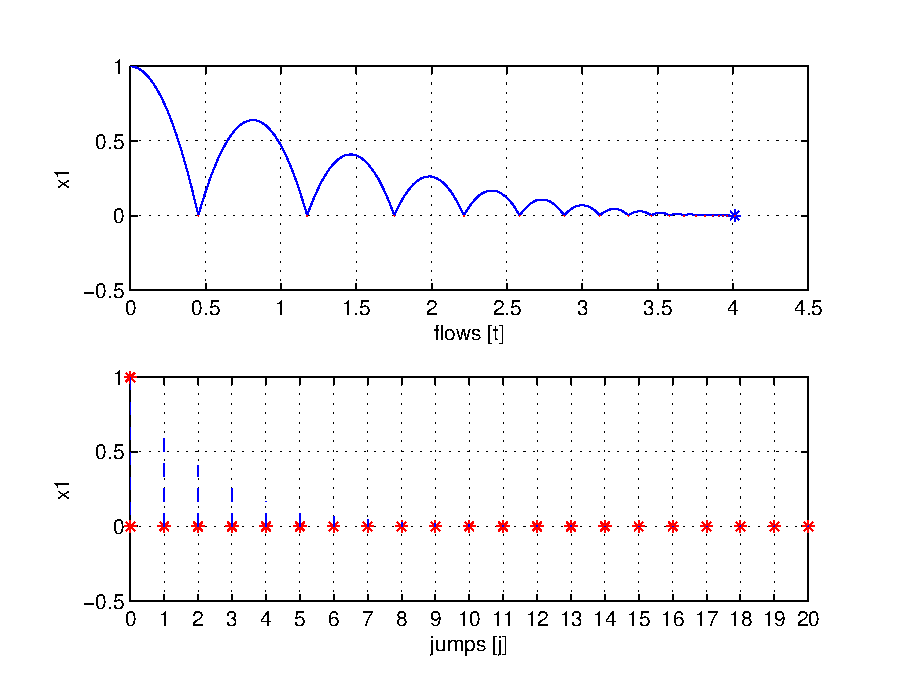
\includegraphics[width=.45\textwidth]{figures/Examples/FlowsAndJumps1lite.eps}
\label{fig:lite-1}}
\qquad
\subfigure[Velocity]{
    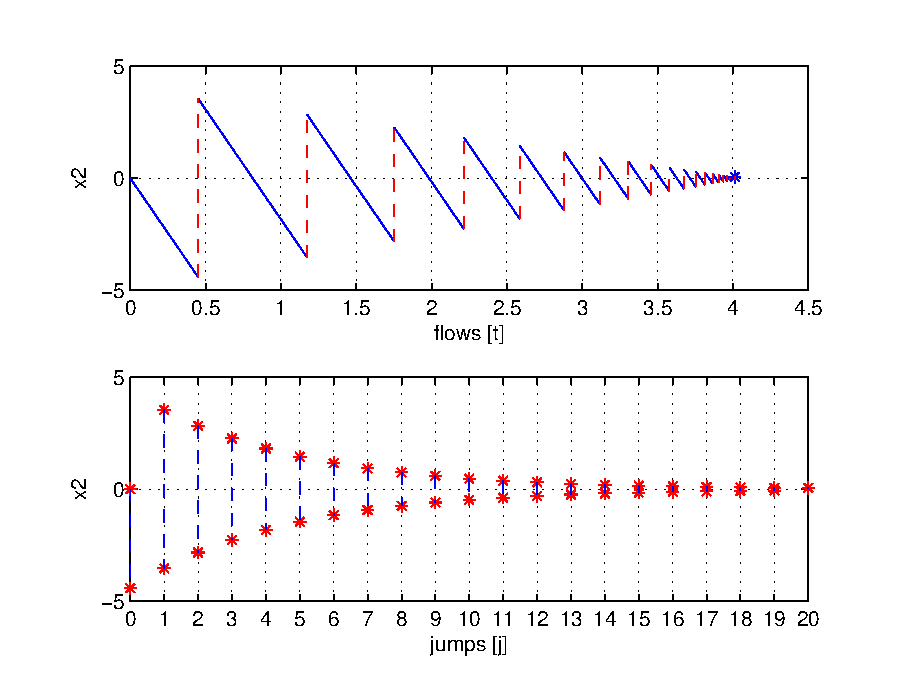
\includegraphics[width=.45\textwidth]{figures/Examples/FlowsAndJumps2lite.eps}
\label{fig:lite-2}}
\caption{Solution of Example \ref{ex:bblite}}
\end{figure}

\begin{figure}[ht]
  \begin{center}
  \psfrag{t}[c]{$t$}
  \psfrag{j}[c]{$j$}
  \psfrag{x1}[c]{$x_1$}
    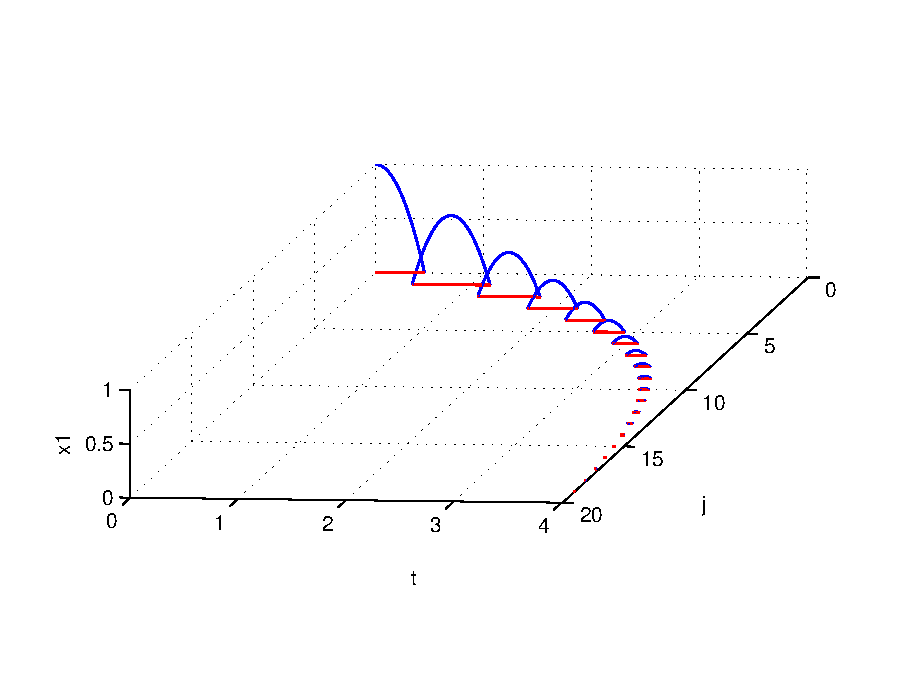
\includegraphics[width=.8\textwidth]{figures/Examples/HybridArclite.eps}
   \caption{Hybrid arc corresponding to a solution of Example~\ref{ex:bblite}: height}
\label{fig:lite-3}
  \end{center}
\end{figure}

A solution to the bouncing ball system from $x(0,0)=[1,0]^\top$ and with $TSPAN = [0 \hspace{2mm} 10], JSPAN = [0 \hspace{2mm} 20]$, $rule =1$, is depicted in Figure~\ref{fig:lite-1} (height) and Figure~\ref{fig:lite-2} (velocity).  Both the projection onto $t$ and $j$ are shown. Figure~\ref{fig:lite-3} depicts the corresponding hybrid arc for the position state.

For MATLAB files of this example, see Examples/Example\_\ref{ex:bblite}.

\end{example}


%% ADDED DETAILS OF \matlab{}-based CODE
\subsection{Solver Function}

%\ricardo{Perhaps add some text here to briefly describe what the functions implement?}

The solver function {\tt HyEQsolver} solves the hybrid system using 
three different functions as shown below. 
First, the flows are calculated using the built-in ODE solver function {\tt ODE45} in \matlab{}. 
If the solution leaves the flow set {\tt C}, the discrete event is detected using 
the function {\tt zeroevents} as shown in Section \ref{sec:eventsdetection}. When the state jumps, 
the next value of the state is calculated via the jump map {\tt g} using the function {\tt jump} 
as shown in Section \ref{sec:jumpmap}.\\

\codeLocation{Matlab2tex} 
% \code{HyEQsolver\_inst.m}
% % % This file was automatically created from the m-file 
% "m2tex.m" written by USL. 
% The fontencoding in this file is UTF-8. 
%  
% You will need to include the following two packages in 
% your LaTeX-Main-File. 
%  
% \usepackage{color} 
% \usepackage{fancyvrb} 
%  
% It is advised to use the following option for Inputenc 
% \usepackage[utf8]{inputenc} 
%  
  
% definition of matlab colors: 
\definecolor{mblue}{rgb}{0,0,1} 
\definecolor{mgreen}{rgb}{0.13333,0.5451,0.13333} 
\definecolor{mred}{rgb}{0.62745,0.12549,0.94118} 
\definecolor{mgrey}{rgb}{0.5,0.5,0.5} 
\definecolor{mdarkgrey}{rgb}{0.25,0.25,0.25} 
  
\DefineShortVerb[fontfamily=courier,fontseries=m]{\$} 
\DefineShortVerb[fontfamily=courier,fontseries=b]{\#} 
  
\begin{Verbatim}[commandchars=\$\{\},numbers=left,numbersep=2pt] 

    $textcolor{mblue}{function} [t j x] = HyEQsolver(f,g,C,D,x0,TSPAN,JSPAN,rule,options,solver,E) 
    $textcolor{mgreen}{%HYEQSOLVER solves hybrid equations.} 
    $textcolor{mgreen}{%   Syntax: [t j x] = HYEQSOLVER(f,g,C,D,x0,TSPAN,JSPAN,rule,options,solver,E)} 
    $textcolor{mgreen} 
    $textcolor{mgreen} 
    $textcolor{mgreen}{%   where x is the state, f is the flow map, g is the jump map, C is the} 
    $textcolor{mgreen}{%   flow set, and D is the jump set. It outputs the state trajectory (t,j)} 
    $textcolor{mgreen}{%   -> x(t,j), where t is the flow time parameter and j is the jump} 
    $textcolor{mgreen} 
    $textcolor{mgreen} 
    $textcolor{mgreen}{%   TSPAN = [TSTART TFINAL] is the time interval. JSPAN = [JSTART JSTOP] is} 
    $textcolor{mgreen}{%       the interval for discrete jumps. The algorithm stop when the first} 
    $textcolor{mgreen} 
    $textcolor{mgreen}{%   rule (optional parameter) - rule for jumps} 
    $textcolor{mgreen}{%       rule = 1 (default) -> priority for jumps rule = 2 -> priority for} 
    $textcolor{mgreen} 
    $textcolor{mgreen}{%   options (optional parameter) - options for the solver see odeset f.ex.} 
    $textcolor{mgreen}{%       options = odeset('RelTol',1e-6);} 
    $textcolor{mgreen} 
    $textcolor{mgreen}{%   solver (optional parameter. String) - selection of the desired ode} 
    $textcolor{mgreen}{%       solver. All ode solvers are suported, exept for ode15i.  See help} 
    $textcolor{mgreen} 
    $textcolor{mgreen}{%   E (optional parameter) - Mass matrix [constant matrix | function_handle]} 
    $textcolor{mgreen}{%       For problems: } 
    $textcolor{mgreen}{%       E*\dot{x} = f(x) x \in C } 
    $textcolor{mgreen}{%       x^+ = g(x)  x \in D} 
    $textcolor{mgreen}{%       set this property to the value of the constant mass matrix. For} 
    $textcolor{mgreen}{%       problems with time- or state-dependent mass matrices, set this} 
    $textcolor{mgreen}{%       property to a function that evaluates the mass matrix. See help} 
    $textcolor{mgreen} 
    $textcolor{mgreen} 
    $textcolor{mgreen}{%         % Consider the hybrid system model for the bouncing ball with data given in} 
    $textcolor{mgreen}{%         % Example 1.2. For this example, we consider the ball to be bouncing on a} 
    $textcolor{mgreen}{%         % floor at zero height. The constants for the bouncing ball system are} 
    $textcolor{mgreen}{%         % \gamma=9.81 and \lambda=0.8. The following procedure is used to} 
    $textcolor{mgreen}{%         % simulate this example in the Lite HyEQ Solver:} 
    $textcolor{mgreen}{%} 
    $textcolor{mgreen}{%         % * Inside the MATLAB script run_ex1_2.m, initial conditions, simulation} 
    $textcolor{mgreen}{%         % horizons, a rule for jumps, ode solver options, and a step size} 
    $textcolor{mgreen}{%         % coefficient are defined. The function HYEQSOLVER.m is called in order to} 
    $textcolor{mgreen}{%         % run the simulation, and a script for plotting solutions is included.} 
    $textcolor{mgreen}{%         % * Then the MATLAB functions f_ex1_2.m, C_ex1_2.m, g_ex1_2.m, D_ex1_2.m} 
    $textcolor{mgreen}{%         % are edited according to the data given below.} 
    $textcolor{mgreen}{%         % * Finally, the simulation is run by clicking the run button in} 
    $textcolor{mgreen}{%         % run_ex1_2.m or by calling run_ex1_2.m in the MATLAB command window.} 
    $textcolor{mgreen}{%} 
    $textcolor{mgreen}{%         % For further information, type in the command window:} 
    $textcolor{mgreen} 
    $textcolor{mgreen}{%         % Define initial conditions} 
    $textcolor{mgreen}{%         x1_0 = 1;} 
    $textcolor{mgreen}{%         x2_0 = 0;} 
    $textcolor{mgreen} 
    $textcolor{mgreen}{%         % Set simulation horizon} 
    $textcolor{mgreen}{%         TSPAN = [0 10];} 
    $textcolor{mgreen} 
    $textcolor{mgreen}{%         % Set rule for jumps and ODE solver options} 
    $textcolor{mgreen} 
    $textcolor{mgreen}{%         % rule = 1 -> priority for jumps} 
    $textcolor{mgreen} 
    $textcolor{mgreen}{%         % rule = 2 -> priority for flows} 
    $textcolor{mgreen} 
    $textcolor{mgreen}{%         % set the maximum step length. At each run of the} 
    $textcolor{mgreen}{%         % integrator the option 'MaxStep' is set to} 
    $textcolor{mgreen}{%         % (time length of last integration)*maxStepCoefficient.} 
    $textcolor{mgreen}{%         %  Default value = 0.1} 
    $textcolor{mgreen}{%} 
    $textcolor{mgreen} 
    $textcolor{mgreen} 
    $textcolor{mgreen}{%         % Simulate using the HYEQSOLVER script} 
    $textcolor{mgreen}{%         % Given the matlab functions that models the flow map, jump map,} 
    $textcolor{mgreen}{%         % flow set and jump set (f_ex1_2, g_ex1_2, C_ex1_2, and D_ex1_2} 
    $textcolor{mgreen}{%         % respectively)} 
    $textcolor{mgreen}{%} 
    $textcolor{mgreen}{%         [t j x] = HYEQSOLVER( @f_ex1_2,@g_ex1_2,@C_ex1_2,@D_ex1_2,...} 
    $textcolor{mgreen} 
    $textcolor{mgreen}{%         % plot solution} 
    $textcolor{mgreen}{%} 
    $textcolor{mgreen}{%         figure(1) % position} 
    $textcolor{mgreen}{%         clf} 
    $textcolor{mgreen}{%         subplot(2,1,1),plotflows(t,j,x(:,1))} 
    $textcolor{mgreen}{%         grid on} 
    $textcolor{mgreen} 
    $textcolor{mgreen}{%         subplot(2,1,2),plotjumps(t,j,x(:,1))} 
    $textcolor{mgreen}{%         grid on} 
    $textcolor{mgreen} 
    $textcolor{mgreen}{%         figure(2) % velocity} 
    $textcolor{mgreen}{%         clf} 
    $textcolor{mgreen}{%         subplot(2,1,1),plotflows(t,j,x(:,2))} 
    $textcolor{mgreen}{%         grid on} 
    $textcolor{mgreen} 
    $textcolor{mgreen}{%         subplot(2,1,2),plotjumps(t,j,x(:,2))} 
    $textcolor{mgreen}{%         grid on} 
    $textcolor{mgreen} 
    $textcolor{mgreen}{%         % plot hybrid arc} 
    $textcolor{mgreen}{%         } 
    $textcolor{mgreen}{%         figure(3)} 
    $textcolor{mgreen}{%         plotHybridArc(t,j,x)} 
    $textcolor{mgreen}{%         xlabel('j')} 
    $textcolor{mgreen}{%         ylabel('t')} 
    $textcolor{mgreen} 
    $textcolor{mgreen}{%         % plot solution using plotHarc and plotHarcColor} 
    $textcolor{mgreen}{%} 
    $textcolor{mgreen}{%         figure(4) % position} 
    $textcolor{mgreen}{%         clf} 
    $textcolor{mgreen}{%         subplot(2,1,1), plotHarc(t,j,x(:,1));} 
    $textcolor{mgreen}{%         grid on} 
    $textcolor{mgreen}{%         ylabel('x_1 position')} 
    $textcolor{mgreen}{%         subplot(2,1,2), plotHarc(t,j,x(:,2));} 
    $textcolor{mgreen}{%         grid on} 
    $textcolor{mgreen} 
    $textcolor{mgreen}{%} 
    $textcolor{mgreen}{%         % plot a phase plane} 
    $textcolor{mgreen}{%         figure(5) % position} 
    $textcolor{mgreen}{%         clf} 
    $textcolor{mgreen}{%         plotHarcColor(x(:,1),j,x(:,2),t);} 
    $textcolor{mgreen}{%         xlabel('x_1')} 
    $textcolor{mgreen}{%         ylabel('x_2')} 
    $textcolor{mgreen} 
    $textcolor{mgreen}{%--------------------------------------------------------------------------} 
    $textcolor{mgreen}{% Matlab M-file Project: HyEQ Toolbox @  Hybrid Systems Laboratory (HSL),} 
    $textcolor{mgreen}{% https://hybrid.soe.ucsc.edu/software} 
    $textcolor{mgreen}{% http://hybridsimulator.wordpress.com/} 
    $textcolor{mgreen}{% Filename: HYEQSOLVER.m} 
    $textcolor{mgreen}{%--------------------------------------------------------------------------} 
    $textcolor{mgreen}{%   See also HYEQSOLVER, PLOTARC, PLOTARC3, PLOTFLOWS, PLOTHARC,} 
    $textcolor{mgreen}{%   PLOTHARCCOLOR, PLOTHARCCOLOR3D, PLOTHYBRIDARC, PLOTJUMPS.} 
    $textcolor{mgreen}{%   Copyright @ Hybrid Systems Laboratory (HSL),} 
    $textcolor{mgreen}{%   Revision: 0.0.0.4 Date: 04/6/2017 16:26:00} 
     
     
    $textcolor{mblue}{if} ~exist($textcolor{mred}{'rule'},$textcolor{mred}{'var'}) 
        rule = 1; 
    $textcolor{mblue}{end} 
     
    $textcolor{mblue}{if} ~exist($textcolor{mred}{'options'},$textcolor{mred}{'var'}) 
        options = odeset(); 
    $textcolor{mblue}{end} 
    $textcolor{mblue}{if} exist($textcolor{mred}{'E'},$textcolor{mred}{$textcolor{mred}{'var'}}) && ~exist($textcolor{mred}{'solver'},$textcolor{mred}{$textcolor{mred}{'var'}}) 
        solver = $textcolor{mred}{'ode15s'}; 
    $textcolor{mblue}{end} 
    $textcolor{mblue}{if} ~exist($textcolor{mred}{'solver'},$textcolor{mred}{'var'}) 
        solver = $textcolor{mred}{'ode45'}; 
    $textcolor{mblue}{end} 
    $textcolor{mblue}{if} ~exist($textcolor{mred}{'E'},$textcolor{mred}{'var'}) 
        E = []; 
    $textcolor{mblue}{end} 
    $textcolor{mgreen}{% mass matrix (if existent)} 
    isDAE = false; 
    $textcolor{mblue}{if} ~isempty(E) 
        isDAE = true; 
        $textcolor{mblue}{switch} isa(E,$textcolor{mred}{'function_handle'}) 
            $textcolor{mblue}{case} true $textcolor{mgreen}{% Function E(x)} 
                M = E; 
                options = odeset(options,$textcolor{mred}{'Mass'},M,$textcolor{mred}{'Stats'},$textcolor{mred}{'off'},... 
                    $textcolor{mred}{'MassSingular'},$textcolor{mred}{'maybe'},$textcolor{mred}{'MStateDependence'},$textcolor{mred}{'strong'},... 
                    $textcolor{mred}{'InitialSlope'},f_hdae(x0,TSPAN(1)));  
            $textcolor{mblue}{case} false $textcolor{mgreen}{% Constant double matrix} 
                M = double(E); 
                options = odeset(options,$textcolor{mred}{'Mass'},M,$textcolor{mred}{'Stats'},$textcolor{mred}{'off'},... 
                    $textcolor{mred}{'MassSingular'},$textcolor{mred}{'maybe'},$textcolor{mred}{'MStateDependence'},$textcolor{mred}{'none'}); 
        $textcolor{mblue}{end} 
    $textcolor{mblue}{end} 
     
    odeX = str2func(solver); 
    nargf = nargin(f); 
    nargg = nargin(g); 
    nargC = nargin(C); 
    nargD = nargin(D); 
     
     
     
    $textcolor{mgreen}{% simulation horizon} 
    tstart = TSPAN(1); 
    tfinal = TSPAN(end); 
    jout = JSPAN(1); 
    j = jout(end); 
     
    $textcolor{mgreen}{% simulate} 
    tout = tstart; 
    [rx,cx] = size(x0); 
    $textcolor{mblue}{if} rx == 1 
        xout = x0; 
    $textcolor{mblue}{elseif} cx == 1 
        xout = x0.'; 
    $textcolor{mblue}{else} 
        error($textcolor{mred}{'Error, x0 does not have the proper size'}) 
    $textcolor{mblue}{end} 
     
    $textcolor{mgreen}{% Jump if jump is prioritized:} 
    $textcolor{mblue}{if} rule == 1 
        $textcolor{mblue}{while} (j<JSPAN(end)) 
            $textcolor{mgreen}{% Check if value it is possible to jump current position} 
            insideD = fun_wrap(xout(end,:).',tout(end),j,D,nargD); 
            $textcolor{mblue}{if} insideD == 1 
                [j $textcolor{mred}{tout jout xout] = jump(g,j,tout,jout,xout,nargg);} 
            $textcolor{mblue}{else} 
                break; 
            $textcolor{mblue}{end} 
        $textcolor{mblue}{end} 
    $textcolor{mblue}{end} 
    fprintf($textcolor{mred}{'Completed: %3.0f%%'},0); 
    $textcolor{mblue}{while} (j < JSPAN(end) && tout(end) < TSPAN(end)) 
        options = odeset(options,$textcolor{mred}{'Events'},@(t,x) zeroevents(x,t,j,C,D,... 
            rule,nargC,nargD)); 
        $textcolor{mgreen}{% Check if it is possible to flow from current position} 
        insideC = fun_wrap(xout(end,:).',tout(end),j,C,nargC); 
        $textcolor{mblue}{if} insideC == 1 
            $textcolor{mblue}{if} isDAE 
                options = odeset(options,$textcolor{mred}{'InitialSlope'},f(xout(end,:).',tout(end))); 
            $textcolor{mblue}{end} 
            [t,x] = odeX(@(t,x) fun_wrap(x,t,j,f,nargf),[tout(end) tfinal],... 
                xout(end,:).', $textcolor{mred}{options);} 
            nt = length(t); 
            tout = [tout; t]; 
            xout = [xout; x]; 
            jout = [jout; j*ones(1,nt)']; 
        $textcolor{mblue}{end} 
         
        $textcolor{mgreen}{%Check if it is possible to jump} 
        insideD = fun_wrap(xout(end,:).',tout(end),j,D,nargD); 
        $textcolor{mblue}{if} insideD == 0 
            break; 
        $textcolor{mblue}{else} 
            $textcolor{mblue}{if} rule == 1 
                $textcolor{mblue}{while} (j<JSPAN(end)) 
                    $textcolor{mgreen}{% Check if it is possible to jump from current position} 
                    insideD = fun_wrap(xout(end,:).',tout(end),j,D,nargD); 
                    $textcolor{mblue}{if} insideD == 1 
                        [j $textcolor{mred}{tout jout xout] = jump(g,j,tout,jout,xout,nargg);} 
                    $textcolor{mblue}{else} 
                        break; 
                    $textcolor{mblue}{end} 
                $textcolor{mblue}{end} 
            $textcolor{mblue}{else} 
                [j $textcolor{mred}{tout jout xout] = jump(g,j,tout,jout,xout,nargg);} 
            $textcolor{mblue}{end} 
        $textcolor{mblue}{end} 
        fprintf($textcolor{mred}{'\b\b\b\b%3.0f%%'},max(100*j/JSPAN(end),100*tout(end)/TSPAN(end))); 
    $textcolor{mblue}{end} 
    t = tout; 
    x = xout; 
    j = jout; 
    fprintf($textcolor{mred}{'\nDone\n'}); 
    $textcolor{mblue}{end} 
      
\end{Verbatim}  
  
\UndefineShortVerb{\$} 
\UndefineShortVerb{\#} 
 
% \label{scr:HyEQsolver}

% \subsubsection{Events Detection}
% \label{sec:eventsdetection}

% \code{zeroevents\_inst.m}
% % % This file was automatically created from the m-file 
% "m2tex.m" written by USL. 
% The fontencoding in this file is UTF-8. 
%  
% You will need to include the following two packages in 
% your LaTeX-Main-File. 
%  
% \usepackage{color} 
% \usepackage{fancyvrb} 
%  
% It is advised to use the following option for Inputenc 
% \usepackage[utf8]{inputenc} 
%  
  
% definition of matlab colors: 
\definecolor{mblue}{rgb}{0,0,1} 
\definecolor{mgreen}{rgb}{0.13333,0.5451,0.13333} 
\definecolor{mred}{rgb}{0.62745,0.12549,0.94118} 
\definecolor{mgrey}{rgb}{0.5,0.5,0.5} 
\definecolor{mdarkgrey}{rgb}{0.25,0.25,0.25} 
  
\DefineShortVerb[fontfamily=courier,fontseries=m]{\$} 
\DefineShortVerb[fontfamily=courier,fontseries=b]{\#} 
  
\begin{Verbatim}[commandchars=\$\{\},numbers=left,numbersep=2pt] 

    $textcolor{mblue}{function} [value,isterminal,direction] = zeroevents(x,t,j,C,D,rule,nargC,nargD) 
    $textcolor{mblue}{switch} rule 
        $textcolor{mblue}{case} 1 $textcolor{mgreen}{% -> priority for jumps} 
            isterminal(1) = 1; $textcolor{mgreen}{% InsideC} 
            isterminal(2) = 1; $textcolor{mgreen}{% Inside(C \cap D)} 
            isterminal(3) = 1; $textcolor{mgreen}{% OutsideC} 
            direction(1) = -1; $textcolor{mgreen}{% InsideC} 
            direction(2) = -1; $textcolor{mgreen}{% Inside(C \cap D)} 
            direction(3) =  1; $textcolor{mgreen}{% OutsideC} 
        $textcolor{mblue}{case} 2 $textcolor{mgreen}{%(default) -> priority for flows} 
            isterminal(1) = 1; $textcolor{mgreen}{% InsideC} 
            isterminal(2) = 0; $textcolor{mgreen}{% Inside(C \cap D)} 
            isterminal(3) = 1; $textcolor{mgreen}{% OutsideC} 
            direction(1) = -1; $textcolor{mgreen}{% InsideC} 
            direction(2) = -1; $textcolor{mgreen}{% Inside(C \cap D)} 
            direction(3) =  1; $textcolor{mgreen}{% OutsideC} 
    $textcolor{mblue}{end} 
     
    insideC = fun_wrap(x,t,j,C,nargC); 
    insideD = fun_wrap(x,t,j,D,nargD); 
    outsideC = -fun_wrap(x,t,j,C,nargC); 
     
     
    value(1) = 2*insideC; 
    value(2) = 2-insideC - insideD; 
    value(3) = 2*outsideC; 
     
    $textcolor{mblue}{end} 
      
\end{Verbatim}  
  
\UndefineShortVerb{\$} 
\UndefineShortVerb{\#} 
 
% \label{scr:zeroevents}

% \subsubsection{Jump Map}
% \label{sec:jumpmap}

% \code{jump\_inst.m}
% % % This file was automatically created from the m-file 
% "m2tex.m" written by USL. 
% The fontencoding in this file is UTF-8. 
%  
% You will need to include the following two packages in 
% your LaTeX-Main-File. 
%  
% \usepackage{color} 
% \usepackage{fancyvrb} 
%  
% It is advised to use the following option for Inputenc 
% \usepackage[utf8]{inputenc} 
%  
  
% definition of matlab colors: 
\definecolor{mblue}{rgb}{0,0,1} 
\definecolor{mgreen}{rgb}{0.13333,0.5451,0.13333} 
\definecolor{mred}{rgb}{0.62745,0.12549,0.94118} 
\definecolor{mgrey}{rgb}{0.5,0.5,0.5} 
\definecolor{mdarkgrey}{rgb}{0.25,0.25,0.25} 
  
\DefineShortVerb[fontfamily=courier,fontseries=m]{\$} 
\DefineShortVerb[fontfamily=courier,fontseries=b]{\#} 
  
\noindent          
 \hspace*{-1.6em}{\scriptsize 1}$  $\color{mblue}$function$\color{black}$ [j tout jout xout] = jump(g,j,tout,jout,xout,nargfun)$\\
 \hspace*{-1.6em}{\scriptsize 2}$  $\color{mgreen}$% Jump$\color{black}$$\\
 \hspace*{-1.6em}{\scriptsize 3}$  j = j+1;$\\
 \hspace*{-1.6em}{\scriptsize 4}$  y = fun_wrap(xout(end,:).',tout(end),jout(end),g,nargfun); $\\
 \hspace*{-1.6em}{\scriptsize 5}$  $\color{mgreen}$% Save results$\color{black}$$\\
 \hspace*{-1.6em}{\scriptsize 6}$  tout = [tout; tout(end)];$\\
 \hspace*{-1.6em}{\scriptsize 7}$  xout = [xout; y.'];$\\
 \hspace*{-1.6em}{\scriptsize 8}$  jout = [jout; j];$\\
 \hspace*{-1.6em}{\scriptsize 9}$  $\color{mblue}$end$\color{black}$$\\
 \hspace*{-2em}{\scriptsize 10}$  $\\ 
  
\UndefineShortVerb{\$} 
\UndefineShortVerb{\#}
% \label{scr:jump}

% \subsubsection{Function Wrapper}
% \label{sec:funwrapp}

% \code{fun\_wrap\_inst.m}
% % % This file was automatically created from the m-file 
% "m2tex.m" written by USL. 
% The fontencoding in this file is UTF-8. 
%  
% You will need to include the following two packages in 
% your LaTeX-Main-File. 
%  
% \usepackage{color} 
% \usepackage{fancyvrb} 
%  
% It is advised to use the following option for Inputenc 
% \usepackage[utf8]{inputenc} 
%  
  
% definition of matlab colors: 
\definecolor{mblue}{rgb}{0,0,1} 
\definecolor{mgreen}{rgb}{0.13333,0.5451,0.13333} 
\definecolor{mred}{rgb}{0.62745,0.12549,0.94118} 
\definecolor{mgrey}{rgb}{0.5,0.5,0.5} 
\definecolor{mdarkgrey}{rgb}{0.25,0.25,0.25} 
  
\DefineShortVerb[fontfamily=courier,fontseries=m]{\$} 
\DefineShortVerb[fontfamily=courier,fontseries=b]{\#} 
  
\begin{Verbatim}[commandchars=\$\{\},numbers=left,numbersep=2pt] 

    $textcolor{mblue}{function} xdelta = fun_wrap(x,t,j,h,nargfun) 
    $textcolor{mgreen}{%fun_wrap   Variable input arguments function (easy use for users).} 
    $textcolor{mgreen}{%   fun_wrap(x,t,j,h,nargfun) depending on the function h written by the} 
    $textcolor{mgreen}{%   user, this script selects how the HyEQ solver should call that} 
    $textcolor{mgreen}{%   function.} 
    $textcolor{mgreen}{%    x: state} 
    $textcolor{mgreen}{%    t: time} 
    $textcolor{mgreen}{%    j: discrete time} 
    $textcolor{mgreen}{%    h: function handle} 
    $textcolor{mgreen}{%    nargfun: number of input arguments of function h    } 
    $textcolor{mgreen}{%--------------------------------------------------------------------------} 
    $textcolor{mgreen}{% Matlab M-file Project: HyEQ Toolbox @  Hybrid Systems Laboratory (HSL), } 
    $textcolor{mgreen}{% https://hybrid.soe.ucsc.edu/software} 
    $textcolor{mgreen}{% http://hybridsimulator.wordpress.com/} 
    $textcolor{mgreen}{% Filename: fun_wrap.m} 
    $textcolor{mgreen}{%--------------------------------------------------------------------------} 
    $textcolor{mgreen}{%   See also HYEQSOLVER, PLOTARC, PLOTARC3, PLOTFLOWS, PLOTHARC,} 
    $textcolor{mgreen}{%   PLOTHARCCOLOR, PLOTHARCCOLOR3D, PLOTHYBRIDARC, PLOTJUMPS.} 
    $textcolor{mgreen}{%   Copyright @ Hybrid Systems Laboratory (HSL),} 
    $textcolor{mgreen}{%   Revision: 0.0.0.3 Date: 01/28/2016 5:12:00} 
     
     
    $textcolor{mblue}{switch} nargfun 
        $textcolor{mblue}{case} 1 
            xdelta = h(x); 
        $textcolor{mblue}{case} 2 
            xdelta = h(x,t); 
        $textcolor{mblue}{case} 3 
            xdelta = h(x,t,j);         
    $textcolor{mblue}{end} 
    $textcolor{mblue}{end}  
\end{Verbatim}  
  
\UndefineShortVerb{\$} 
\UndefineShortVerb{\#} 
 
% \label{scr:funwrapp}


\section{Acknowledgments}
\label{sec:acknowledgments}

We would like to thank Giampiero Campa for his thoughtful feedback 
and advice as well as Torstein Ingebrigtsen Bo for his comments 
and initial version of the \matlab{}-based simulator code, 
and the following list of people who have helped to test this toolbox:

\begin{itemize}
\item Cenk Oguz Saglam - University of California, Santa Barbara
\item Bharani Malladi - The University of Arizona
\end{itemize}

\bibliographystyle{unsrt} 
\bibliography{biblio}\label{sec:refs}

\include{foot}

\end{document}
